% Created 2018-08-07 Di 12:51
\documentclass{scrartcl}

%\usepackage[latin1]{inputenc}
\usepackage[utf8]{inputenc}
\usepackage[T1]{fontenc}
\usepackage{fixltx2e}
\usepackage{graphicx}
\usepackage{longtable}
\usepackage{float}
\usepackage{wrapfig}
\usepackage{rotating}
\usepackage[normalem]{ulem}
\usepackage{amsmath}
\usepackage{textcomp}
\usepackage{marvosym}
\usepackage{wasysym}
\usepackage{amssymb}
\usepackage{hyperref}
\tolerance=1000
\author{Simon Pfaff}
\date{\today}
\title{Master Thesis}
\hypersetup{
  pdfkeywords={},
  pdfsubject={},
  pdfcreator={Emacs 24.5.1 (Org mode 8.2.6)}}
\begin{document}

\begin{center}
\thispagestyle{empty}
\textbf{\huge Master Thesis}\\[2mm]
\textbf{\huge Seperating the good from the bad... Exploring the genomic landscape of chloroplasts from genomic sequencing data}\\[5mm]
\textbf{\LARGE }\\[3mm]
{\LARGE Simon Pfaff}\\[2mm]

\includegraphics[width=.7\linewidth]{./neuSIEGEL.pdf}
{\large Julius-Maximilians-Universität Würzburg}\\[1mm]
{\large Fakultät für Biologie}
\end{center}
\cleardoublepage
\
\thispagestyle{empty}
\maketitle
\begin{center}
\textbf{Seperating the good from the bad... Exploring the genomic landscape of chloroplasts from genomic sequencing data}

\includegraphics[width=.5\linewidth]{./neuSIEGEL.pdf}\\[1cm]
{\large Julius-Maximilians-Universität Würzburg}\\
{\large Betreuer: Dr. Markus Ankenbrand}\\
{\large Betreuer: Prof. Dr. Jörg Schulz}\\
{\large Betreuer: Dr. Frank Förster}\\
{\large Lehrstuhl für Bioinformatik}\\
{\large Center for Computational and Theoretical Biology}
\setcounter{page}{1}
\clearpage
\end{center}
\tableofcontents
\clearpage
\section{Zusammenfassung / Abstract}
\label{sec-1}
\subsection{Deutsch}
\label{sec-1-1}
In der Heutigen Big Data Ära, werden immer mehr neue Daten erzeugt. Doch können auch bereits vorhandene Daten durchaus noch Informationen enthalten welche bisher ungenutzt sind.
Dank der Open Science sind viele dieser Daten frei verfügbar. In diesem Konkreten Falle werden verschiedene Programme verwendet um in pflanzlichen Genom Daten, Chloroplasten Genome zu 
suchen. Chloroplasten haben ihre eigene zirkuläre DNA, und wenn beim Sequenzieren diese nicht gefiltert wurde, dann ist sie noch in den Daten vorhanden. So kann man ohne 
eine neue Sequenzierung machen zu müssen Chloroplasten DNA für Analysen erhalten. Es wurden verschiedene Programme getestet und verglichen, um so viele Chloroplasten 
wie nur möglich zu bauen und damit Analysen durchzuführen. Es wurde eine vollautomatische Pipeline erstellt mit denen Chloroplasten Genome einfach aus Pflanzen Genomen
extrahiert werden können. 
\subsection{English}
\label{sec-1-2}
In to days Big Data Era every day new data is created. But this is not necessary to get new information. In older data oftentimes hides other data, which may not be used till today.
Since open science is growing in the last years many of this data is freely accessible. In this case plant whole genome data is used. This data oftentimes includes chloroplast
genome data, when in the sequencing process nobody removed it, by cell nucleus extraction. There were different tools which provided a suit to extract this chloroplast genome data from plant
genome data. They were tested, compared and the best were used to calculate a lot of chloroplast genomes. This chloroplast genomes got analysed with different methods. Also there is now
a fully automatic pipeline for chloroplast genome extraction from genomic sequencing data.
\clearpage

\section{Einleitung}
\label{sec-2}
\subsection{Chloroplasten}
\label{sec-2-1}
Chloroplasten sind extrem wichtig, ein Großteil der Pflanzen, vor allem grün Pflanzen besitzen diese und nutzen sie um Energie durch Photosynthese zu erzeugen\footnote{Purves Biologie, Sadava D, Hillis D.M, Heller H.C, Berenbaum M.R, (9. Auflage S. 14)}.
Ihr Genom gilt als hoch konserviert, sowohl in der Gen Orientierung als auch dem Gen Inhalt \footnote{Raubeson L, Jansen R. (2005). Chloroplast genomes of plants, Plant diversity and evolution: genotypic and phenotypic variation in higher plants. Diversity and Evolution of Plants-Genotypic and Phenotypic Variation in Higher Plants. 3. \url{10.1079/9780851999043.0045}.}, dieser besteht zwischen 100 und 200 Genen\footnote{Howe CJ. (2016). Chloroplast Genome. In eLS, John Wiley \& Sons,  \url{10.1002/9780470015902.a0002016.pub3}}. 
Die DNA des Chloroplasten hat in etwa eine Konturlänge von 30 bis 60 Mikrometer und besitzt eine Masse von ungefähr 80 - 130 Millionen daltons\footnote{Burgess, Jeremy (1989). An introduction to plant cell development. Cambridge: Cambridge university press. S. 62. ISBN 0-521-31611-1.}.
Chloroplasten zeigen
eine auffällige Genom Struktur, das Genom ist ein einem Plasmid welches sich in drei Teile aufteilt. Dem Large Single Copy, dem 
Small Singles Copy, welche beide durch zwei Inverted repeats unterbrochen sind (Fig. 1)\footnote{Shaw J, Lickey EB, Schilling EE, et al. (2007). Comparison of whole chloroplast genome sequences to choose noncoding regions for phylogenetic studies in angiosperms: The tortoise and the hare III. American Journal of Botany. \url{10.3732/ajb.94.3.275}.}. Chloroplasten zeigen eine viel geringere Substitutionsrate
als in genomischer DNA, diese ist noch einmal signifikant geringer in den Inverted repeat Regionen \footnote{Wolfe KH, Li WH, Sharp PM. (1988). Rates of nucleotide substitution vary greatly among plant mitochondrial, chloroplast and nuclear DNA. Proc Natl Acad Sci USA \url{10.1073/pnas.84.24.9054}.}. Dennoch zeigen sich
Einzelnucleotid-Polymorphismen (SNPs)\footnote{1001 Genomes Consortium, (2016) 1,135 genomes reveal the global pattern of polymorphism in \emph{Arabidopsis thaliana}. Cell. \url{https://doi.org/10.1016/j.cell.2016.05.063}}. Zudem gibt es ein seltenen Fällen eine Genwanderung von Genen auf dem IR zum SSC, wodurch ein IR weg
fallen kann, sodass solche Chloroplasten nur noch ein IR besitzen \footnote{Jansen RK, Wojciechowski MF, Sanniyasi E, et al. Complete plastid genome sequence of the chickpea (Cicer arietinum) and the phylogenetic distribution of rps12 and clpP intron losses among legumes (Leguminosae). Molecular phylogenetics and evolution. \url{10.1016/j.ympev.2008.06.013}.} . Vor allem in gezüchteten Nutzpflanzen finden sich auch 
Invertierungen des IR \footnote{Palmer JD, Jansen RK, Michaels HJ, et al. (1988).  Chloroplast DNA Variation and Plant Phylogeny. Annals of the Missouri Botanical Garden,  \url{10.2307/2399279}}. Durch ihre hohe Konservierung sind Chloroplasten und ihre Gene sehr gut für Barcoding geeignet\footnote{Song Y, Wang S, Ding Y, et al. (2017) Chloroplast genomic resource of Paris for species discrimination. Sci. Rep. \url{10.1038/s41598-017-02083-7}}. Mit diesem
Barcoding können Pflanzen und ihre Varianten identifiziert werden. Neue Studien zeigen, dass der komplette Chloroplast selbst als ein Art "Ultra-barcode"
verwendet werden könnte, da die Variation in Chloroplasten in einer Spezies doch mehr variiert als angenommen \footnote{Kane N, Sveinsson S, Dempewolf H, et al.(2012), Ultra-barcoding in cacao (Theobroma spp.; Malvaceae) using whole chloroplast genomes and nuclear ribosomal DNA. American Journal of Botany, \url{10.3732/ajb.1100570}}. 
Die Gene auf einem Chloroplasten lassen sich in verschiedene Klassen einteilen (Fig. 2). Zunächst gibt es die Gene welche für die Photosynthese wichtig sind,
hier unterteilt man nochmal in Photosystem I (psaA, psaB, etc.), Photosystem II (psbA, psbB, etc.), Cytochrome b6f (petA, petB,etc.), 
ATP Synthese (atpA, atpB, etc.), RuBisCo(rbcL) und NAD(P)H dehydrogenase Gene(ndhA, ndhB, etc.)\footnote{Ravi V, Khurana JP, Tyagi AK, et al. (2007). An update on chloroplast genome. Plant Systematics and Evolution. \url{10.1007/s00606-007-0608-0}.}. Die zweite Klasse beinhaltet Gene welche für den
Genetischen Apparat, also Transkription, Translation und Replikation nötig sind, sowie RNA Gene. Hierzu zählen Transfer RNA (trnH,trnK, etc.), ribosomale RNA (rrn16, rrn5, etc.), 
RNA Polymerasen (rpoA, rpoB, etc.) und ribosomale Gene (rps2, rps3, rpl2, rpl16,etc.). Die dritte und letzte Kategorie beschreibt Gene welche konservierte Open Reading Frames (ORFs) haben und
ycfs (Hypotheticalchloroplast open reading frames) genannt werden sowie potentiell kodierende Gene wie matK und cemA\footnotemark[12]{}. Vor allem stark konservierte Gene wie rbcL und matK und cemA werden 
häufig für Barcoding oder zum berechnen von phylogenetischen Bäume verwendet.
\begin{figure}
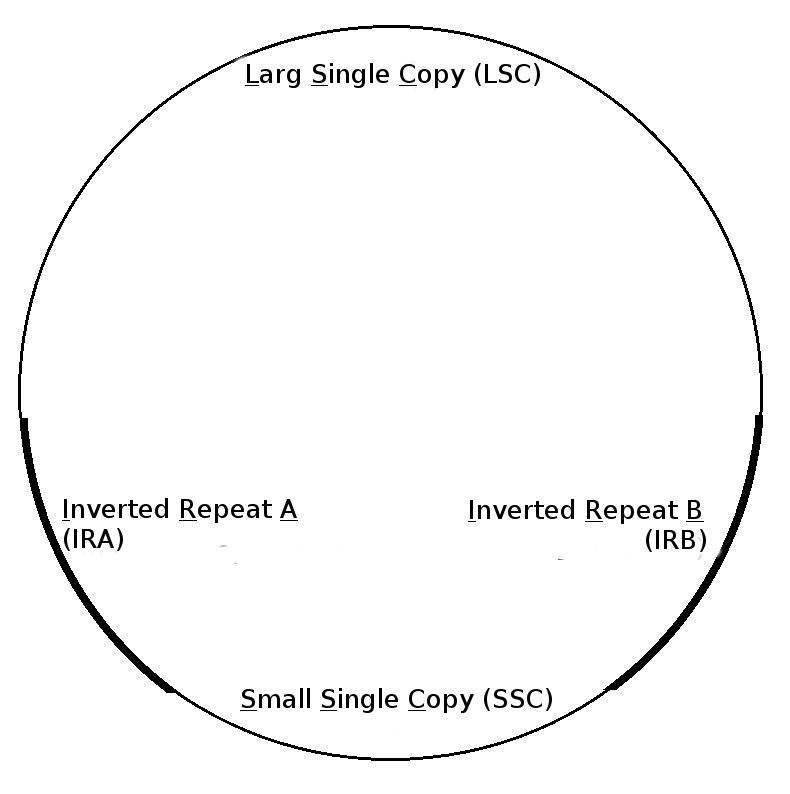
\includegraphics[width=.9\linewidth]{./Chloroplast_1.png}
\caption[Chloroplast Genom Einteilung]{\textbf{Chloroplast Genom Einteilung} Der Chloroplast ist unterteilt in Large Single Copy, Small Single Copy und Inverted Repeat, diese unterteilen sich nochmal in IRA und IRB. LSC und SSC werden jeweils von den IRs unterbrochen.}
\end{figure}

\begin{figure}
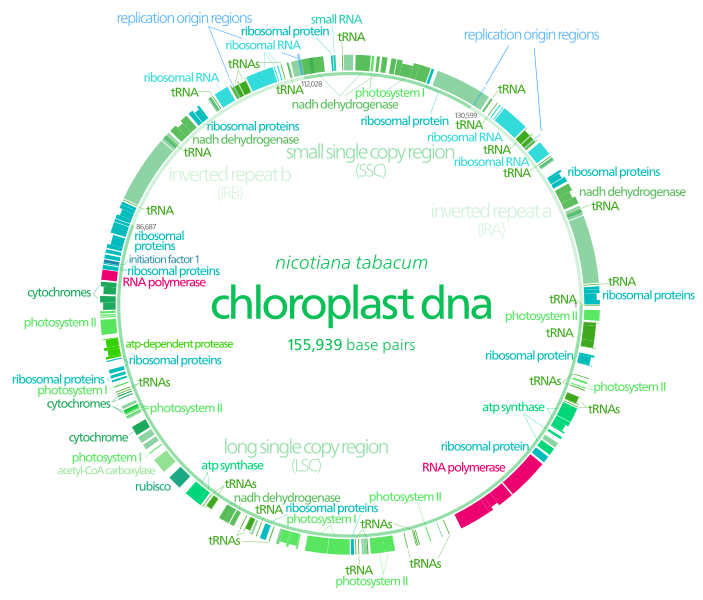
\includegraphics[width=.9\linewidth]{./703px-CtDNA.png}
\caption[Chloroplast Genom: Gen Klassen]{\textbf{Chloroplast Genom: Einteilung Gen Klassen} Das Chloroplast Genom der Tabak pflanze, die innere Beschriftung zeigt den - Strand, die Äußere den + Strand der DNA. Die Kerben visualisieren Introns.Wikipedia unter Wikimedia Commonsen Lizenz\url{https://en.wikipedia.org/wiki/File:CtDNA.svg}}
\end{figure}

\subsection{Big Data}
\label{sec-2-2}
Die Big Data Ära zeichnet sich vor allem durch die Flut an Daten aus, welche kaum noch zu bewältigen ist. Im biologischen Sinne zeichnet sich diese 
Flut an Daten vor allem durch genomische Daten aus. Durch sogenannte Hochdurchsatz Methoden in modernen Sequenzierungs Technologien wie PacBio\footnote{\url{https://www.pacb.com/}} oder Illumina\footnote{\url{https://www.illumina.com/}}
sie verwenden, können sehr viele genomische Daten in kurzer Zeit für vergleichsweise wenig Geld erzeugt werden. Um dieser Daten Herr zu werden sind vor allem
Programme die diese Daten auswerten wichtig. Die Anforderung an diese Programme sind unter anderem eine hohe Geschwindigkeit und vor allem eine hohe 
Automatisierbarkeit. Um solche Programme zu entwickeln sind vor allem Kenntnisse in Informatik und in Biologie notwendig. Kenntnisse in Informatik
werden benötigt um Programme sinnvoll zu strukturieren und diese anschließend in einer geeigneten Programmiersprache zu erstellen. Zudem müssen diese
Programme immer wieder gewartet werden. Auch könnten neue Features eingebaut werden oder dass Programm nochmals Optimiert werden. Kenntnisse in der Biologie
werden benötigt um biologische Fragestellungen sowie Sachverhalte zu verstehen. Diese müssen korrekt in das Programm implementiert werden, zudem müssen 
natürlich alle Ergebnisse korrekt interpretiert werden. Nur mit Kenntnissen in beiden Fächern können Programme welche in der Biologie und Bioinformatik verwendet
werden effektiv erstellt und gewartet werden.  
\subsection{Open Science}
\label{sec-2-3}
Mit der Flut der ansteigenden Daten wächst in den letzten Jahren auch immer mehr die Akzeptanz zur "Open Science".
"Open Science" bezeichnet eine Bewegung welche fordert, dass Wissenschaft und alles was dazugehört, Daten, Programme, Ergebnisse öffentlich und für jedermann 
zugänglich sein soll. Befürworter dieser Bewegung argumentieren damit, dass Wissen für jedermann zugänglich sein sollte, und nicht nur für Ausgewählte oder gar
gegen Bezahlung. So steigere sich unter anderem die Akzeptanz der Wissenschaft als auch deren Glaubwürdigkeit. Da die Ergebnisse von jedem nachvollziehbar 
veröffentlicht werden müssen, mit allen Rohdaten und Vorgehensweisen. Dies sei der eigentliche Gedanke hinter der Wissenschaft, sie solle jedem zugänglich sein.
Diese Bewegung findet vor allem bei jung Wissenschaftler aber auch bei Älteren immer mehr Anklang. Mittlerweile gibt es mehrere Lizenz Modelle die unter
Open Science laufen. Diese Regeln wie die Daten verwendet werden dürfen oder müssen. Dies reicht von Freigeben der Daten und jeglichem Verwendungszweck bis hin
zum Zwang, dass alles was mit diesen Daten oder auch Programmen veröffentlicht wird wieder unter der gleichen Open Source Lizenz zu publizieren ist.
Alle hier verwendeten Programme und Daten sind unter Open Source Lizenzen veröffentlicht, sonnst wäre diese Arbeit gar nicht möglich. 
Deswegen werden alle Ergebnisse wiederum öffentlich verwendbar sein. Open Science sollte keine Bewegung sein, sondern einfach nur Science.\footnote{Watson M. (2015) When will ‘open science’ become simply ‘science’?, Genome Biology \url{https://doi.org/10.1186/s13059-015-0669-2}}


\subsection{Daten in Daten}
\label{sec-2-4}
Bei den heutzutage geringen Kosten, Daten vor allem genomische Daten, zu erzeugen ist es nicht verwunderlich dass immer neue Daten generiert werden.
Dennoch steckt in bereits erhobenen Daten meist mehr Information als zunächst verwendet. In genomischen Daten zum Beispiel, hier findet sich meistens Daten 
von Organellen, wie Mitochondrien oder Chloroplasten, welche ihre eigene DNA besitzen. Diese sind dort zu finden da vor einer Sequenzierung häufig keine 
Kern Extraktion durchgeführt wird, da diese mehr Zeit und Geld kosten würde. Diese Organellen DNA können mit bestimmten Programmen gefiltert werden, hierfür 
wurde unter anderem der chloroExtractor\footnote{Ankenbrand MJ, Pfaff S, Förster F, et al., (2018). chloroExtractor: extraction and assembly of the chloroplast genome from whole genome shotgun data. Journal of Open Source Software, \url{https://doi.org/10.21105/joss.00464}}\textsuperscript{,}\,\footnote{\url{https://github.com/chloroExtractorTeam/chloroExtractor}} programmiert. Dieser kann in genomischen Pflanzen Daten Chloroplasten DNA finden und diese verwenden um einen vollständigen
Chloroplasten zu bauen. Hiermit müssen somit keine neuen Sequenzierungen für Chloroplasten mehr durchgeführt werden, wenn man an Chloroplasten forschen möchte.
\subsection{Bestehende Programme und ihre Ansätze}
\label{sec-2-5}
Es gibt verschiedene Ansätze um Chloroplasten Genome bzw. ihre DNA aus genomischen Pflanzen Daten zu extrahieren. Die wohl einfachste Möglichkeit ist ein Referenz basiertes
Mapping der Daten auf einen Referenz Chloroplasten. Hierzu muss lediglich ein nah verwandter Chloroplast als Referenz benutzt werden. So können die Reads, welche auf diese Referenz
passen genommen werden und assembliert werden, mit der gleichen Referenz. Dies funktioniert allerdings nur wenn man eine passende Referenz benutzt, diese sollte von der gleichen Spezies oder
zumindest einer Nah verwandten Spezies stammen. Ein anderer Ansatz besteht darin den Chloroplasten de novo zu assemblieren, also ohne Referenz. Um diesen Ansatz zu benutzen müssen
aber zunächst die Reads mit Chloroplasten Genom aus den Daten gezogen werden. Hier gibt es wiederum verschiedene Möglichkeiten. Eine Möglichkeit ist es die Reads gegen eine Datenbank
von Chloroplasten Genen zu blasten, hierzu muss entweder eine Datenbank von Chloroplasten Genen gestellt werden oder der Benutzer muss eine Pseudo-Referenz einen sogenannten Seed angeben.
Ein Seed, was von einigen Basenpaaren bis zu einem kompletten Chloroplasten reichen kann, kann auch eingesetzt werden um durch ein reines Mapping Reads zu finden. Bei kleinen Seeds wird dieser
häufig durch gefundene Reads erweitert und eine Liste von Seed erstellt. Auch hier muss aber sichergestellt werden, dass der Seed in den Chloroplasten Daten vorhanden ist.
Von diesen Methoden gibt es auch Abwandlungen, wie z.b. das scannen der Daten durch Kmers, hier werden die Daten in verschiedene Kmers zerteilt, durch plotten dieser Kmers können
an spezifischen Stellen überrepräsentierte Kmers gefunden werden, diese überrepräsentierten Kmer spiegeln häufig Plastome wieder. Diese sind unter anderem Chloroplasten aber auch
Mitochondrien, sie besitzen ihre eigene DNA und kommen im Schnitt häufiger vor als DNA welche im Zellkern zu finden ist. Allerdings gibt es weitaus mehr DNA welche durch häufiges vorkommen
überrepräsentiert sind in einem Kmer Plot, hierzu gehören rRNA Gene, Transposons und andere genomische Repeats, welche je nach Art und Spezies variieren kann. 
Da der chloroExtractor einen Kmer basierten Ansatz benutzt ist ein solches idealisiertes Kmer Diagramm in dessen Logo zu finden(Fig. 3).
\begin{figure}
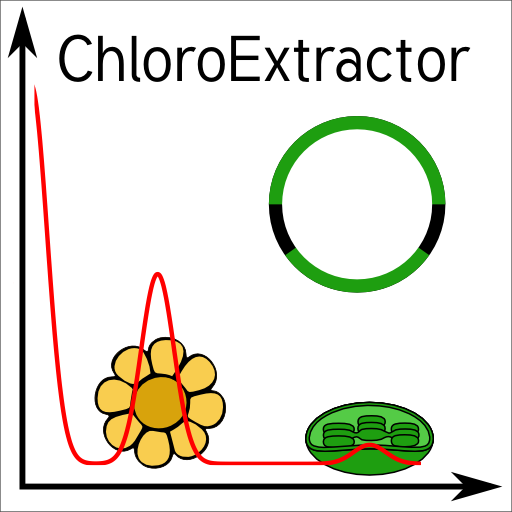
\includegraphics[width=.6\linewidth]{./logo512.png}
\caption[chloroExtractors Logo]{\textbf{chloroExtractor Logo} Das Logo des chloroExtractors zeigt die Verteilung der Genomischen Daten in einem Kmer Plot. Der erste Peak zeigt die Kmers Pflanzengenom, der zweite kleinere Peak zeigt die Kmers mit Chloroplasten Genom.}
\end{figure}
Abgesehen von den Ansätzen der Programme gibt es zwei verschiedene Arten von Programmen per se, die einen benutzen bereits vorhandene Programme wie Assambler, Mapper oder Kmer-counter. Diese 
Bauen eine Pipeline um diese Programme, sodass diese in der richtigen Reihenfolge mit den richtigen Parametern mit nur einem Befehl gesteuert werden können. Der Vorteil ist, solche Programme
sind einfacher zu warten da sie meist kleiner sind als Programme die dies nicht tun und einfacher zu Programmieren. Allerdings sind sie von diesen drittanbieter Programmen abhängig und es können Probleme 
auftreten wenn diese Änderungen bzw. Updates ausgeben, weswegen meist die kompatiblen Versionen angegeben werden. Ein weiterer Nachteil, der Benutzer muss häufig weitere Programme, sogenannte Abhängigkeiten installieren
bevor er das eigentliche Programm nutzen kann. Die andere Möglichkeit ist es die komplette Maschinerie selbst zu Programmieren, dies ist sehr aufwendig und bedeutet viel Wartungsarbeit. Vorteil hier
ist das keine anderen Abhängigkeiten benötigt werden außer ein System welches das Programm verwenden kann. In dieser Arbeit wurden verschiedene Typen von Programmen verwendet.
Es wurden von allen Programmen die jeweils neusten Versionen benutzt, und wenn es zu großen Änderungen wie Bug-fixes kam auf die neuere Version gewechselt, um das bestmögliche Ergebnis für die Daten
zu erhalten.
\subsubsection{chloroExtractor}
\label{sec-2-5-1}
Der chloroExtractor (Versionen: 1.0.2, 1.0.3, 1.0.4 ) \footnotemark[16]{}\textsuperscript{,}\,\footnotemark[17]{} ist ein Programm welches durch eine Kombination aus Kmer Analyse und Mapping auf bekannte Chloroplasten Gene, Reads von Chloroplasten aus Pflanzen Sequenzierungs Daten
extrahiert. Es wurde 2018 vom chloroExtractorTeam veröffentlicht \footnotemark[16]{} und besteht hauptsächlich aus Perl und R Code. Es verwendet ein Pipeline Programm (PipeWrap.pm\footnote{\url{https://github.com/BioInf-Wuerzburg/perl5lib-PipeWrap}}) um den richtigen Ablauf zu steuern.
Dieses Pipeline Tool wird durch eine Konfigurationsdatei gesteuert, sodass ein Benutzer einfach neue Schritte einfügen könnte. Auch können hiermit einfach über eine Datei, Parameter gesteuert werden welche dann in 
allen verwendeten Programmen gleich sind. Es könnt so auch einzelnen Programmen speziellen Input mitgegeben werden. Auch verfügt der chloroExtractor dank PipeWrap über ein Checkpoint System. Bricht der Ablauf des Programms
ab, kann er am genau diesem Punkt wieder gestartet werden ohne das Programm von neu starten zu müssen. Zunächst verwendet der chloroExtractor Bowtie2 \footnote{Langmead B, Salzberg S. (2012), Fast gapped-read alignment with Bowtie 2. Nature Methods, \url{9:357-359}.} um die Reads auf eine Referenz aus codierenden Chloroplasten Gene zu mappen.
Hierdurch wird der relative Anteil an Chloroplasten geschätzt. Durch ein R Skript wird der Datensatz auf 200-fache Chloroplasten Reads Coverage skaliert. Anschließend wird iterativ durch Jellyfish \footnote{Marcais G, Kingsford C.(2011), A fast, lock-free approach for efficient parallel counting of occurrences of k-mers. Bioinformatics  \url{10.1093/bioinformatics/btr011}} Kmere erzeugt und jene mit
zu niedriger Coverage aussortiert. Die Kmere die im richtigen Coverage Bereich liegen werden anschließend mit SPAdes\footnote{Bankevich A, Nurk S, Antipov D, et al. (2012), SPAdes: A New Genome Assembly Algorithm and Its Applications to Single-Cell Sequencing, Journal of Computational Biology, \url{10.1089/cmb.2012.0021}} assembliert , SPAdes arbeitet de novo und benötigt
keine Referenz. SPAdes verwendet eine De Brujin-Graphen Methode um die Reads richtig zusammen zu fügen, diese werden dann durch ein Perl Skript (fcg.pl) zu einem zirkulären Chloroplasten zusammengebaut. Dieses Skript überprüft
gleichzeitig mit BLAST+\footnote{Camacho C, Coulouris G, Avagyan V, et al. (2009), Selecting control genes for RT-QPCR using public microarray data, BMC Bioinformatics \url{https://doi.org/10.1186/1471-2105-10-42}} ob es sich bei den ausgegebenen Reads wirklich um Chloroplasten handelt (Fig. 4). Falls es dazu kommt
das SPAdes den Chloroplasten nicht komplett zusammenbauen kann, dann gibt das fcg.pl Skript die Contigs, welches für den Chloroplasten verwendet werden aus. Hier gibt es verschiedene Fälle. Kann nur die Zirkularität 
des Chloroplasten nicht aufgelöst werden gibt der chloroExtractor LSC, SSC und IR aus. Sind gar keine Verbindungen der Contigs möglich gibt das fcg.pl Skript jene Contigs aus die einen BLAST+ Treffer besitzen und somit ein
teil des Chloroplasten sind.  Es wurden drei Verschiedene Versionen des chloroExtractors verwendet, dies brachten unter anderem Bug fixes welche das 
Programm zum Absturz brachten. Aber auch Verbesserungen am fcg.pl Skript.

\begin{figure}
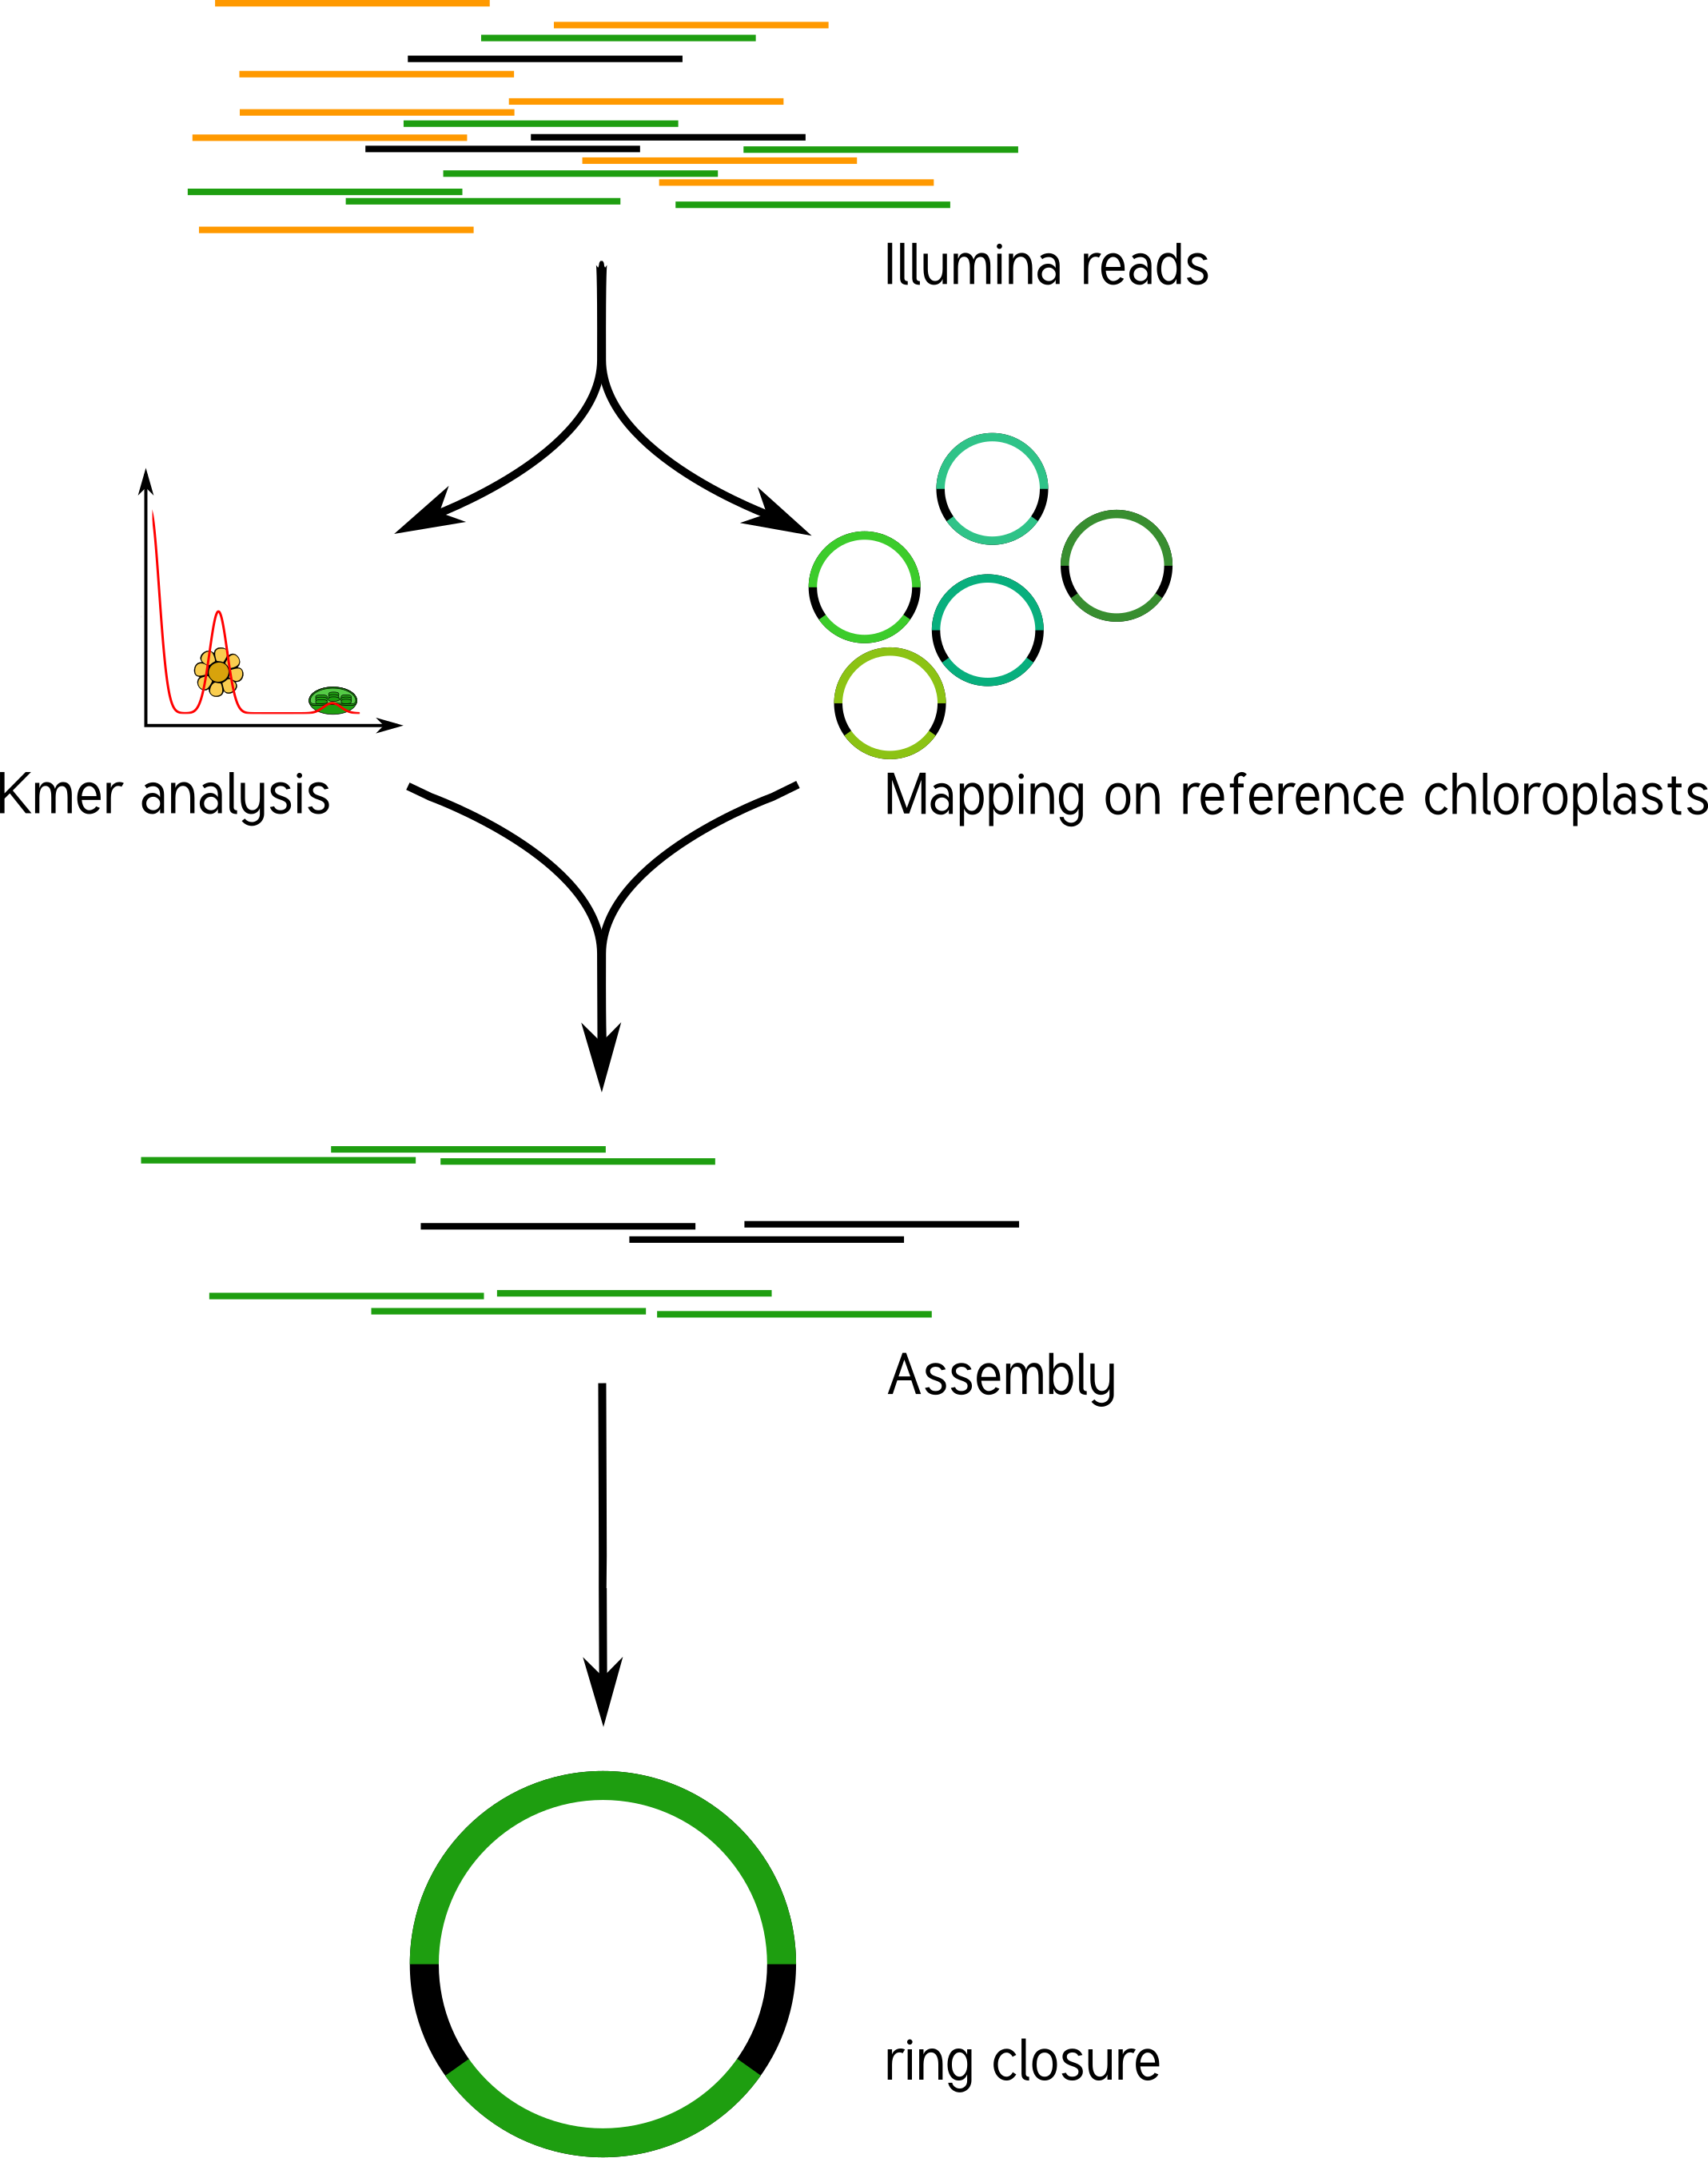
\includegraphics[width=.9\linewidth]{./workflow.png}
\caption[Ablauf des chloroExtractors]{\textbf{Ablauf des chloroExtractors} Eine Kombination aus Kmer Analyse und Mapping auf bekannte Chloroplasten rekrutieren Chloroplasten reads um diese anschließend zu Assemblieren um anschließend einen Ringschluss herbeizuführen. (Ankenbrand et al., (2018).)}
\end{figure}

\subsubsection{fast-plast}
\label{sec-2-5-2}
Fast-plast  (Version: 1.2.8) \footnote{\url{https://github.com/mrmckain/Fast-Plast}} ist ein weiteres Programm, welches verwendet wird um Chloroplasten DNA zu finden. Es ist in Perl und in C++ programmiert und verwendet auch SPAdes, 
aber zusätzlich Bowtie1 sowie Bowtie2. Auch hier wird Blast+ verwendet um die richtigen Reads zu finden. 
\subsubsection{NOVOPlasty}
\label{sec-2-5-3}
Im Gegensatz zu den anderen verwendeten Programmen, benutzt NOVOPlasty (Versionen: 2.6.8. 2.6.9, 2.7.0 )\footnote{\url{https://github.com/ndierckx/NOVOPlasty}}\textsuperscript{,}\,\footnote{Dierckxsens N, Mardulyn P , Smits G. (2016), NOVOPlasty: De novo assembly of organelle genomes from whole genome data. Nucleic Acids Research, \url{10.1093/nar/gkw955}} keine drittanbieter Programme. Es benötigt somit keine Abhängigkeiten von anderen Programmen
und ist komplett in Perl programmiert. NOVOPlasty benutzt sogenannte Seeds um Chloroplasten DNA zu finden, dies können einzelne Chloroplasten Gene sein, aber auch ein kompletter Chloroplast.
Die Verschiedenen Verwendeten Versionen versprachen Bug fixes sowie neue Features. 
\subsubsection{Org.ASM}
\label{sec-2-5-4}
Org.ASM ( Version: 1.0.00-alpha11) \footnote{\url{https://pythonhosted.org/ORG.asm/}} ist ein Programm hauptsächlich geschrieben in Python. Es versucht überrepräsentierte Sequenzen zu finden und diese zu assemblieren\footnote{\url{https://git.metabarcoding.org/org-asm/org-asm/wikis/home}}. 
Mit Hilfe eines Seeds versucht er diese Sequenzen zu finden.Chloroplasten und andere Organellen wie Mitochondrien sind in Zellen überrepräsentiert, vor allem
wenn man eine geringe Coverage über das Pflanzen Genom hat, somit sind diese detektierbar\footnote{\url{https://pythonhosted.org/ORG.asm/algorithms.html}}.
\subsubsection{GetOrganelle}
\label{sec-2-5-5}
GetOrganelle (Versionen: 1.9.82, 1.0.1, 1.0.3 )\footnote{\url{https://github.com/Kinggerm/GetOrganelle}}\textsuperscript{,}\,\footnote{Jin J, Yu W, Yang J, Song Y, et al. (2018), GetOrganelle: a simple and fast pipeline for de novo assembly of a complete circular chloroplast genome using genome skimming data. bioRxiv, \url{http://doi.org/10.1101/256479}} verwendet zum lokalisieren der Chloroplasten Reads ähnlich wie andere Programme Bowtie2 \footnotemark[19]{} und Blast+, nur muss hier eine Referenz mitgegeben werden. 
Diese wird nur hierfür
verwendet, das assemblieren hingegen geschieht de novo mit SPAdes. Wie auch beim chloroExtractor wird hier der fastg-Graph verwendet um den Chloroplasten zu finden, aber dies muss in falle 
des GetOrganelle per Hand, mit Hilfe des Programms Bandage\footnote{Wick RR, Schultz .B, Zobel J, et al (2015). Bandage: interactive visualisation of de novo genome assemblies. Bioinformatics, \url{https://doi.org/10.1093/bioinformatics/btv383}} vollzogen werden. Wie bereits erwähnt nutzt der chloroExtractor ein Perl Skript welchen diesen händischen Schritt automatisiert.(Fig. 5) 
Vom GetOrganelle wurden drei Versionen verwendet. Zunächst 1.9.82, diese wurde geändert zu 1.0.1 (github commit: b390260 vom 31. März 2018) und 1.0.3. In den Verschiedenen Versionen gab es diverse Bug Fixes, sowie
kleine Features.
Zudem wurde das Programm GetOrganelle mit 1.0.1 in einer Wissenschaftlichen Arbeit veröffentlicht \footnotemark[30]{}.
\subsubsection{IOGA}
\label{sec-2-5-6}
Der Iterative Organellar Genome Assambly, kurz IOGA (Keine Versionsnummer vergeben, github commit: c460ea9 vom 10. Sep. 2016 )\footnote{\url{https://github.com/holmrenser/IOGA}}\textsuperscript{,}\,\footnote{Bakker FT, Lei D, et al. (2015), Herbarium genomics: plastome sequence assembly from a range of herbarium specimens using an Iterative Organelle Genome Assembly pipeline, Biol. J. Linnean Soc. \url{https://doi.org/10.1111/bij.12642}} verwendet BBmap \footnote{\url{https://jgi.doe.gov/data-and-tools/bbtools/}} für das filtern und trimmen der reads, um anschließend mit 
SOAPdenovo2 \footnote{Luo R, Liu B, Xie Y, et al. (2012), SOAPdenovo2: an empirically improved memory-efficient short-read de novo assembler. GigaScience.  \url{10.1186/2047-217X-1-18}.} und SPAdes \footnotemark[21]{} die Reads zu assemblieren. 
Auch dieses Programm benötigt eine Referenz. Der IOGA ist in Python geschrieben.
\begin{figure}
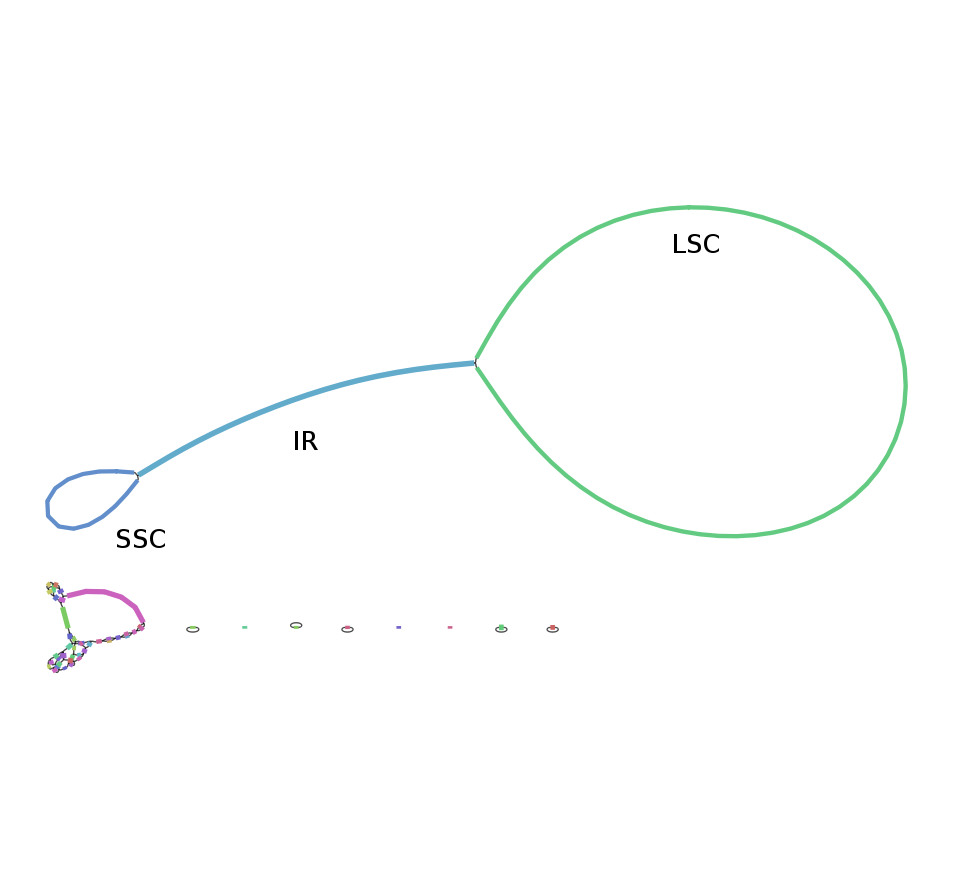
\includegraphics[width=.9\linewidth]{./graphCE_SRR1945473_1.png}
\caption[Bandage - Fastg Visualisierung]{\textbf{Bandage - Fastg Visualisierung} Die Visualisierung einer fastg Datei, der eigentlich zirkuläre Chloroplast zeigt sich in einer Form in der SSC (Blau) und LSC (Grün) durch eine Kette welche den IR (Türkis) darstellt verbunden sind. Diese Form wird im fcg.pl Skript des chloroExtractors aufgelöst, wobei beim GetOrganelle diese Struktur per Hand gefunden werden muss.}
\end{figure}
\subsection{Interesse an Chloroplasten, was tun damit mit diesen Daten?}
\label{sec-2-6}
Mit der steigenden Anzahl an frei erhältlichen Chloroplasten Genomen, welche aus NCBI oder CpBase geladen werden können und gegen Ende 2016 erstmals die 1000 Genome überschritten haben\footnote{Tonti-Filippini J, Nevill PG, Dixon K, et al. (2017), What can we do with 1000 plastid genomes?. Plant J, \url{10.1111/tpj.13491}} können immer mehr Versuche mit vielen Chloroplasten durchgeführt werden.
So ist immer noch nicht geklärt wie genau die Replikation von Plastid Genomen wie von Chloroplasten wirklich funktioniert. Wie werden Mutationen im Inverted Repeat repariert oder bei der Replikation auf beide IRs übernommen?
Da SNPs im IR immer auf beiden gefunden werden. Welche Mutationen treten am häufigsten auf und wie sind diese evtl. an die Struktur des Genoms gekoppelt \footnote{Massouh A, Schubert J, Yaneva-Roder L, et al. (2016), Spontaneous Chloroplast Mutants Mostly Occur by Replication Slippage and Show a Biased Pattern in the Plastome of Oenothera. The Plant Cell. \url{10.1105/tpc.15.00879}.}? Auch ist immer noch nicht exakt verstanden wie Chloroplasten
vererbt werden, es wird zwar angenommen das diese ähnlich wie Mitochondrien maternal vererbt werden doch gibt es bei Pflanzen auch viele Arten die biparental oder uniparental Chloroplasten vererben\footnote{Greiner S, Sobanski J, Bock R. (2015), Why are most organelle genomes transmitted maternally? Bioessays. \url{10.1002/bies.201400110}.}. Die in den letzten 
Jahren stark steigende Anzahl an Chloroplasten Genomen gibt diesen Fragestellungen immer mehr neue Rohdaten die diese Fragen lösen könnten. Auch Probleme die nur mit kleinen Änderungen im Chloroplasten Genom zu tun 
haben (SNPs)
können so auf den Grund gegangen werden, oder auch die Adaption von verschiedenen Chloroplasten Genen in das Pflanzengenom und der daraus folgenden Änderung im Photosynthese Systems\footnote{Wicke S, Schneeweiss GM, dePamphilis CW, et al. (2011) The evolution of the plastid chromosome in land plants: gene content, gene order, gene function. Plant Molecular Biology.  \url{10.1007/s11103-011-9762-4}.}. Auch kann ohne große Änderung an der
kodierenden Sequenz, alleine durch Änderung an Transkriptionsfaktoren oder deren Level viel Einfluss auf solche Systeme genommen werden, welche natürlich auch mit dem Chloroplasten zusammenhängen\footnotemark[36]{}. Wie bereits erwähnt 
eigenen sich Chloroplasten gut als Barcode Marker. Auch hier können Fortschritte mit mehr Daten erlangt werden. Zudem können mit vielen Chloroplasten Daten sehr gut Phylogenetische Bäume berechnet werden\footnote{Chase MW, Fay MF. (2001) Ancient flowering plants: DNA sequences and angiosperm classification. Genome Biology. \url{https://doi.org/10.1186/gb-2001-2-4-reviews1012}}.
Dies sind alles Beispiele wie zwischen vielen Spezies mit Hilfe von Chloroplasten Forschung betrieben werden kann. Aber auch innerhalb einer Spezies tauchen Variabilitäten auf, und dies konnte nur mit vielen verschiedenen
Chloroplasten der gleichen Spezies herausgefunden werden. So wurden beim 1001 Genom Projekt mehrere Tausend SNPs auf \emph{A.thaliana} Chloroplasten gecalled\footnote{\url{http://1001genomes.org/}}\textsuperscript{,}\,\footnotemark[7]{}. 
Doch können nicht nur viele Chloroplasten Probleme lösen, schon einzelne neue Chloroplasten können sehr aufschlussreich und informativ sein. So wurde die Idee des chloroExtractors z.B. nur aus dem Grund
entworfen einen Chloroplasten aus dem Dionaea muscipula ( Venusfliegenfalle ) Genom zu extrahieren, um diesen separat zu haben, um das Genom leichter zu assemblieren und annotieren. Denn es kann durchaus vorkommen
dass bei neuen Genomen, welche de novo assembliert werden müssen, Verunreinigungen durch Chloroplasten auftreten können. Denn \textasciitilde{}5 - 20\% der kompletten DNA wird von Plastiden-DNA ausgemacht, je nach Spezies und Gewebe\footnotemark[36]{}.


\subsection{Aufgaben in der Master Thesis}
\label{sec-2-7}
Die Aufgaben dieser Thesis ist grob in drei Teile eingeteilt. Zunächst sollen die verschiedenen Programme, der chloroExtractor \footnotemark[16]{}\textsuperscript{,}\,\footnotemark[17]{}, fast-plast\footnotemark[23]{}, IOGA\footnotemark[32]{}\textsuperscript{,}\,\footnotemark[33]{}, GetOrganelle\footnotemark[29]{}\textsuperscript{,}\,\footnotemark[30]{},
Org.ASM \footnotemark[26]{}und NOVOPlasty\footnotemark[24]{}\textsuperscript{,}\,\footnotemark[25]{} verglichen werden und herausgefunden werden welche das oder die besten Programme sind um damit so viele Chloroplasten Genome zu erzeugen wie 
möglich. Hier soll vor allem darauf geachtet werden dass die Programme Automatisierbar sind um einen hohen Durchsatz zu haben. Zudem sollen die Programme Ressourcen schonend arbeiten. 
Der zweite Teil ist das Produzieren von Chloroplasten Genomen, hierzu werden die Pflanzen Genome des 1001 Genom Projektes verwendet. Nach internen Besprechungen und ersten Tests des chloroExtractors,
wird angenommen das ca. 10 - 20\%\footnote{Interne Absprachen mit Förster F. und Ankenbrand M. über geschätzte Ergebnisse
\clearpage} der Datensätze einen kompletten Zirkulären Chloroplasten erbringen könnten. Dies hängt von mehreren Variablen ab. Zunächst wie viel Chloroplasten DNA ist in den Daten vorhanden, dies
unterscheidet sich je nachdem welches Gewebe verwendet wurde zum Sequenzieren. Hier haben Wurzeln weniger Chloroplasten als Blüten oder Blätter. Auch hängt es davon ab wie "gut" die Daten sind, generell gilt je 
größer die Reads desto besser zu assemblieren, auch zu beachten sind insert Size und Anzahl der Reads.
Auf den so Produzierten Chloroplasten sollen verschiedene wissenschaftliche Analysen durchgeführt werden, so zum Beispiel eine Varianz Analyse sowie eine Genomweite Assoziationsstudie, kurz GWAS \footnote{Korte A, Farlow A. (2013), The advantages and limitations of trait analysis with GWAS: a review. Plant Methods. \url{10.1186/1746-4811-9-29}.}.
Eine GWAS versucht bestimmte Traits, also Eigenschaften mit Genomischen Varianten zu assoziieren, um anschließend eine Aussage darüber treffen zu können ob diese Variante einen Einfluss auf diese 
Eigenschaft hat oder nicht. Hierzu werden die einzelnen Chromosomen einzeln oder als komplettes Genom angesehen, je nach Ansatz oder Fragestellung.
Auch sollte eine Struktur Varianz Analyse durchgeführt werden. Zudem könnten diese Daten benutzt werden um Chloroplasten besser als Genetische Marker zu benutzen. 
Der dritte Teil ist das Suchen nach bisher noch nicht dokumentierten Chloroplasten Genomen, hierzu sollen Daten verwendet werden welche noch keinen Eintrag in der Chloroplasten Datenbank haben.



\section{Material / Methoden}
\label{sec-3}
\subsection{Evaluation der Programme}
\label{sec-3-1}
Um die oben genannten Programme zu vergleichen habe ich mir verschiedene Ansätze überlegt.
Um zunächst zu testen wie genau die Programme funktionieren und ob diese überhaupt funktionieren,
wurden sie auf dem Testset SRR5216995 (\emph{Arabidopsis thaliana}: Col-0) mit eine Millionen reads getestet, 
dieser ist frei zugänglich bei NCBI und dient als Testset beim chloroExtractor\footnotemark[16]{}. Um eine 
Automatisierung zu erhalten musste für jedes Programm ein Dockercontainer\footnote{\url{https://www.docker.com/}}(s. Anhang Tab.9) gebaut werden, falls dieser nicht 
schon einer vorhanden war, letzteres traf nur für den chloroExtractor zu. Diese Dockercontainer sind auf Dockerhub\footnote{\url{https://hub.docker.com/}} frei
zur Verfügung\footnote{\url{https://hub.docker.com/u/chloroextractorteam/}}. Um das Ziel zu erreichen
so viele Chloroplasten wie möglich zu extrahieren, musste eine Automatisierungslösung für alle Programme
erstellt werden, damit keine evtl. Manuelle Schritte oder Auswertungen der zeitbestimmende Schritt sind.
Um dies zu erreichen mussten zusätzlich einige Bash und Perl Skripte (s. Anhang) geschrieben werden, welche eine volle
Automatisierung ermöglichen.Um für alle Programme, welche einen Seed oder eine Referenz benötigen Chancengleichheit herzustellen wurde hier überall die gleiche Datei verwendet. 
Diese Datei benutzt der chloroExtractor, hier handelt es sich um 4154 Chloroplasten Gene, diese sind aus verschiedenen Arten. Bei den Genen handelt es sich um ndhB, rps12, psbD, rpl2 und psbA. 
Liefert ein Programm seine eigenen Referenzen mit, wie es der chloroExtractor tut, wurden diese nicht geändert. Da diese als Standardparameter gelten, welche nicht verändert werden sollten.   

\subsubsection{Testdaten}
\label{sec-3-1-1}
Es wurden verschiedene Größe von Dateien verwendet. So sind dies alles Illumina short Read Daten, doch unterscheiden sich diese in Readlänge, Insertsize und Anzahl der Reads.

\paragraph{Simulierte Daten}
\label{sec-3-1-1-1}
Um zu Testen wie gut die verschiedenen Programme mit unterschiedlichen Anteilen von Chloroplasten DNA in
Genom Daten zurechtkommen, wurden drei verschiedene Testdatensätze simuliert(Genom : Chloroplast - 1:10, 1:100, 1:1000). 
Mit diesen sollte auch getestet werden ob die Programme mit viel oder wenig Chloroplasten DNA Anteil zurecht kommen oder einen dieser Fälle 
bevorzugen. Um diese Daten vorzubereiten wurden von \emph{Arabidopsis thaliana} (TAIR10 \footnote{\url{https://www.ncbi.nlm.nih.gov/assembly/GCF_000001735.3/}}) die jeweiligen Chromosomen wie auch die Daten
des Chloroplasten von NCBI heruntergeladen. Diese wurden in den jeweiligen Verhältnissen zusammen kopiert.
Diese Testdatensätze wurden mit ART\footnote{Weichun H, Leping L, Jason RM, Gabor TM. (2015), ART: a next-generation sequencing read simulator, Bioinformatics, \url{https://doi.org/10.1093/bioinformatics/btr708}}\textsuperscript{,}\,\footnote{\url{https://www.niehs.nih.gov/research/resources/software/biostatistics/art/index.cfm}}(Version: 2.5.8) erzeugt. ART wird dazu verwendet Short-reads zu erzeugen, ART kann keine zirkulären Daten wie Chloroplasten 
erzeugen, deswegen wurden diese als lineare Sequenzen verwendet mit der Abfolge LSC-IRB-SSC-IRA, mit einem Overlap zwischen IRA und LSC: (IRA)-LSC-IRB-SSC-IRA. 
Mitochondrien DNA wurde nicht mit simuliert, da sich zunächst auf die Chloroplasten fokussiert werden sollte und diese Mitochondrien die Komplexität der Daten
erhöht.
Um die verschiedenen Verhältnisse von Genom und Chloroplasten zu bekommen wurden die Chloroplasten Daten einfach
vervielfältigt und anschließend zusammen kopiert. Hiernach wurden sie mit folgenden ART Kommandos als short Reads simuliert.
Hiernach wurden die Daten gemischt, da es zu Problemen kommt wenn diese Daten sortiert sind. Für diese Daten wurden 150 Basen paare Reads simuliert, 
und eine Coverage der Daten welche 100x beträgt. 
Für die Tests wurden eine Millionen Reads pro Datei benutzt, da diese genug Chloroplasten DNA enthalten sollten.
\\
{\small 'art\_illumina [options] -i <INPUT\_SEQ\_FILE> -l <READ\_LEN> -f <FOLD\_COVERAGE>
-o <OUTPUT\_FILE\_PREFIX> -m <MEAN\_FRAG\_LEN> -s <STD\_DE>'}
\\
\\
'1:10 : ./art\_illumina -p -i sequence-arabidopsis-thaliana-kern-chl-1zu10.fa -l 150 -f 100 
-o a\_thaliana\_1\_10\_sim -m 500 -s 150'
\\
\\
'1:100 :  ./art\_illumina -p -i sequence-arabidopsis-thaliana-kern-chl-1zu100.fa -l 150 -f 100 
-o a\_thaliana\_1\_100\_sim -m 500 -s 150'
\\
\\
'1:1000 :  ./art\_illumina -p -i sequence-arabidopsis-thaliana-kern-chl-1zu1000.fa -l 150 -f 100 
-o a\_thaliana\_1\_1000\_sim -m 500 -s 150'

\paragraph{1001 Genom Projekt}
\label{sec-3-1-1-2}
Um einen ersten Eindruck über die Programme und deren Erfolgs rate zu bekommen wurden parallel zu den Tests mit simulierten Daten, die ersten Tests mit realen Datensätzen vorgenommen. 
Hierzu wurden Daten aus dem 1001 Genom Projekt\footnotemark[41]{} verwendet, dies sind alles Daten von \emph{Arabidopsis thaliana}. Es wurden 11 Datensätze ( SRR1945435 - SRR1945445 ) verwendet. Diese sind alle
frei verfügbar und wurden von NCBI heruntergeladen. Es wurden jeweils zwei Millionen Reads pro Datei gezogen, mit 150 Basenpaaren pro Read. 

\paragraph{GetOrganelle-Paper preprint}
\label{sec-3-1-1-3}
Um zu weitere Testdaten zu ermitteln und ein Urteil darüber zu fällen welche Programme weiter verwendet werden,
wurden 57 Datensätze welche im GetOrganelle Paper \footnotemark[30]{} verwendet wurden
auf allen Programmen getestet. In dieser Arbeit wurden bei 47 Datensätzen von 57, mit
dem GetOrganelle erfolgreich zirkuläre Chloroplasten extrahiert. Diese Daten sind auch frei zugänglich und wurden
von NCBI heruntergeladen. Gerade hier gab es einige Abweichungen in Dateigrößen. Reads reichten von 75 Basenpaaren 
bis zu 300 Basenpaare pro Read. Es wurden hier fünf Millionen Reads pro Datei verwendet, da diese im GetOrganelle Paper
auch verwendet wurden.

\subsubsection{Welche Programme werden weiter verwendet.}
\label{sec-3-1-2}
Um alle Daten aus dem 1001 Genom Projekt (1135 Datensätze) zu berechnen, mussten aufgrund 
von Hardware technischen Limitierungen die besten Programme ausgewählt werden. Diese Programme müssen in
in Geschwindigkeit sowie in Erfolgs- und Fehlerrate überzeugen. Des weiteren müssen diese Programme gut automatisierbar sein, 
d.h. am besten mit nur Befehl gestartet werden können, sodass kein weiterer Aufwand anfällt. Dies gilt
vor allem auch bei der Wahl der Parameter mit denen das Programm gestartet wird. Diese können nicht 
für jeden Datensatz angepasst werden, was bedeutet dass die Standardparameter verwendet werden.
Dies ist notwendig um einen hohen Durchsatz an Berechnungen zu ermöglichen.
\paragraph{Installation \& Automatisierung}
\label{sec-3-1-2-1}
Alle Programme konnten mit Hilfe von einigen Skripts und dem erstellen eines Dockercontainers so 
automatisiert werden, dass sie einen hohen Durchsatz erreichen konnten. Das Einzige Programm welches
einen Händischen Schritt benötigt ist der GetOrganelle, hier muss die fastg Datei in Bandage
geöffnet werden und der zirkuläre Chloroplast selbst heraus gesucht werden.
Bei den verschiedenen Skripts handelt es sich vor allem um Start-Skripts. Aber es mussten auch ein paar 
kleine Skripts verwendet werden um kleine Bugs zu fixen. So kann der IOGA keine Unterordner verwenden da er sonnst
versucht auf Falsche Dateien zuzugreifen und abstürzt. Dies scheint ein Bug in einem Splitt Befehl zu sein. Beim GetOrganelle mussten
zusätzliche Befehle eingebaut werden damit SPAdes keine Fehlermeldungen bringt und abbricht, da er bestimmte Funktionen (hammer.py) nicht ausführen konnte
welche für eine Fehler Korrektur verwendet werden, welche GetOrganelle gar nicht nutzt. Org.ASM konnte nur erfolgreich in einem Dockercontainer
installiert werden, da dieses Programm sonnst verschiedenste Fehlermeldungen brachte. Alle Programme welche Perl verwenden, also
chloroExtractor, fast-plast und NOVOPlasty, brachten Fehlermeldungen, da innerhalb des Dockercontainers Globale Variablen nicht vollständig gesetzt waren. 
Diese Fehler waren aber nicht fatal, und konnten mit dem setzten dieser Variable leicht entfernt werden. 
Für jedes Programm wurde ein Skript geschrieben welches die Laufzeit überprüft und wenn dieses fertig ist, eine Auswertung startet.

\paragraph{Erfolgsrate}
\label{sec-3-1-2-2}
Um zunächst zu überprüfen ob ein wirklich ein kompletter Chloroplast zusammengebaut wurden. Wurde bei den ersten Testdatensätzen ein Referenz Mapping auf
TAIR10 benutzt. Hierzu wurde mit Bowtie2, später mit minimap2\footnote{Li, H. (2018). Minimap2: pairwise alignment for nucleotide sequences. Bioinformatics. \url{10.1093/bioinformatics/bty191}}(Version: 2.10-r761)  der Chloroplast auf das TAIR10 Chloroplasten Genom gemapt. Auch wurde mit AliTV \footnote{Ankenbrand MJ, Hohlfeld S, Förster F, et al. (2017) AliTV—interactive visualization of whole genome comparisons. PeerJ Computer Science, \url{https://doi.org/10.7717/peerj-cs.116}} 
eine Visualisierung des Mappings erstellt. Nachdem klar war das es sich bei allen ausgegeben Daten um Chloroplasten handelt, und weil diese Art der 
Auswertung schlecht Automatisierbar war, wurde ein Bash Skript geschrieben welche die Auswertung übernimmt. Dieses Skript überprüft die Größe des
Chloroplasten und in wie vielen Contigs der Chloroplast ausgegeben wurde. Hierzu wurde das SeqFilter\footnote{\url{https://github.com/BioInf-Wuerzburg/SeqFilter}}(Version: 2.1.8) Skript verwendet, und anschließend über ein Bash
Skript eine Entscheidung getroffen ob es sich um einen kompletten Chloroplasten handelt oder nicht (s. Anhang: Skripte:ev\_stat.sh). Hierzu wurden Verschiedene
Kategorien eingeführt(s. Tab. 1). Diese Auswertung wurde für dann für alle Testdaten sowie die GetOrganelle Preprint Daten verwendet. Zudem gab es zu den vier Kategorien, in denen
Erfolge eingeteilt wurden noch Error, wenn kein Ergebnis vorhanden war wenn das Programm z.B. durch einen Fehler abgebrochen hat. Sowie Cancelled wenn das Programm länger als 14 Tage brauchte 
wurde es abgebrochen.
\begin{table}[!h]
\caption[Erfolgsraten Einteilung]{\textbf{Erfolgsraten Einteilung} Das Skript ev\_stat.sh scannt die Output Dateien und teilt diese je nach Größe und Anzahl der Contigs in verschiedene Kategorien ein. }
\begin{center}
\begin{tabular}{lll}
Kategorie & Contigs & Basenpaare\\
\hline
Success & 1 & 110 kbp - 180 kbp\\
Partial & > 1 & 110 kbp - 180 kbp\\
Incomp:high & > 1 & > 180 kbp\\
Incom:low & > 1 & > 110 kbp\\
 &  & \\
\end{tabular}
\end{center}
\end{table}

\paragraph{Geschwindigkeit}
\label{sec-3-1-2-3}
Einer der weniger entscheidenden aber dennoch wichtigen Punkte nach dem gefiltert wurde ist die Geschwindigkeit, 
oder besser die Laufzeit der Programme. Zunächst wurde hier die Durchschnittszeit genommen, die der Prozess zum rechnen benötigt,
anschließend wurde mit dem time Linux Kommando die CPU als auch die Real-zeit gemessen. Die Geschwindigkeit von Programmen mit vielen Abhängigkeiten 
brauchen im Schnitt länger, da zum benutzen der Dockercontainer Singularity\footnote{\url{https://singularity.lbl.gov/}}(Version: 2.4.5-dist) verwendet wurde. Dieses Benötigt Zeit um den Container zu verwenden,
zudem wird Zeit in Anspruch genommen wenn viele Daten in den Container gemountet werden müssen.
\paragraph{Benötigte Ressourcen}
\label{sec-3-1-2-4}
Ein weiterer Punkt nachdem aussortiert wurde ist der benötigte RAM verbrauch. Es wurden verschiedene Größen von Dateien verwendet
um in Erfahrung zu bringen wie sich dies auf Ressourcen und Laufzeit auswirkt. Zudem wurde zum Ausführen der Dockercontainer 
Singularity \footnotemark[53]{} verwendet, welches die benötigte Laufzeit und die benötigten Ressourcen, wie RAM beeinflusst. 

\subsection{Varianz Analyse}
\label{sec-3-2}
Um mehr über die Chloroplasten und deren Verbreitung, sowie Mutationsrate und somit Varianz zu erfahren wurden zwei verschiedene Varianzanalysen durchgeführt. 
Zunächst sollte überprüft werden welche Einflüsse die Programme und ihre Strategien den Chloroplasten zu assemblieren, speziell deren Assambler, auf die Varianz der 
entstehenden Chloroplasten hat. Hierzu wurden die assamblierten Chloroplasten, welche beide verwendeten Programme gemeinsam hatten verwendet. Diese Läufe wurden zunächst
zehn fach wiederholt, auch um einen Eindruck über die Reproduzierbarkeit der Ergebnisse zu bekommen. Diese Chloroplasten wurden anschließend mit minimap2 \footnotemark[50]{} auf das 
Referenzgenom ( TAIR10 Chloroplast \footnote{\url{https://www.ncbi.nlm.nih.gov/nuccore/NC_000932.1}} ) gemapt. Hiernach wurde eine Varianzanalyse mit Samtools\footnote{Li H, Handsaker B, Wysoker A, et al. (2009) The Sequence alignment/map (SAM) format and SAMtools, Bioinformatics \url{10.1093/bioinformatics/btp352}}(Version: 0.1.19-96b5f2294a) durchgeführt, hierzu wurde der Befehl
'mpileup/bcftools call' \footnote{Li H, (2011) A statistical framework for SNP calling, mutation discovery, association mapping and population genetical parameter estimation from sequencing data, Bioinformatics  \url{10.1093/bioinformatics/btr509}} (bcftools Versionen:0.1.19-96b5f2294a \& 1.8) verwendet. Dieser führt eine Varianzanalyse bzw. ein SNP calling durch. Die zweite Varianzanalyse wurde auf allen Chloroplasten welche aus dem
1001 Genom Projekt gebaut wurden erstellt. Auch diese wurden auf den Referenz Chloroplasten mit minimap2 gemapt und anschließend mit Samtools' 'mpileup' Funktion einem
SNP calling unterzogen. 

\subsection{GWAS}
\label{sec-3-3}
Häufig wird eine GWAS über das komplette Genom berechnet. Doch können auch einzelne Chromosomen oder Organellen bereits signifikante Varianten besitzen. 
So soll mit dieser GWAS der Einfluss von Chloroplasten Varianten auf Eigenschaften der \emph{A.thaliana} getestet werden. Hierzu wurden die SNP callings aus der Varianzanalyse verwendet.
Verschiedene Trait-Tabellen wurden von Arapheno\footnote{\url{https://arapheno.1001genomes.org/}}\textsuperscript{,}\,\footnote{Seren Ü, Grimm D, Fitz J, et al. (2017) AraPheno: a public database for Arabidopsis thaliana phenotypes, Nucleic Acids Research, \url{https://doi.org/10.1093/nar/gkw986}}, einer Trait Datenbank für \emph{A.thaliana}, heruntergeladen und zusammen mit den Varianzanalyse Daten in ein R\footnote{\url{https://www.r-project.org/}} Skript gegeben.
Dieses R Skript nutzt zunächst vcfR\footnote{\url{https://cran.r-project.org/web/packages/vcfR/index.html}}, ein R Paket, um die verschiedenen VCF (Variance Calling File) Daten einzulesen. Anschließend ruft es ein weiteres R Skript auf welches
freundlicher weiße von Korte et. al\footnotemark[43]{} zur Verfügung gestellt wurde und eine GWAS Analyse durchführt.

\subsection{Struktur Varianz Analyse}
\label{sec-3-4}
Wie bereits erwähnt können Chloroplasten auch verschiedene Strukturelle Änderungen evolvieren. Diese sind durch die Rohdaten, welche meist short Reads sind, nicht aufzudecken.
Da diese zu kurz sind um komplette Struktur Varianten zu überspannen.\footnotemark[7]{} Hierzu könnten nun die komplett de novo Assemblierten Chloroplasten verwendet werden.
Es wurde versucht mit Delly\footnote{\url{https://github.com/dellytools/delly}} (Version: v0.7.8) und Breakdancer\footnote{\url{https://github.com/genome/breakdancer}}(Version: 1.3.6) Struktur Varianten in Chloroplasten zu finden.  

\subsection{Neue Chloroplasten}
\label{sec-3-5}
Um neue Chloroplasten von Spezies zu finden, welche noch nicht in der CpBase \footnote{\url{http://rocaplab.ocean.washington.edu/old_website/tools/cpbase}}\textsuperscript{,}\,\footnote{\url{http://rocaplab.ocean.washington.edu/tools/cpbase_test/}} Datenbank sind, wurde eine Liste von Möglichen Daten von NCBI mit CpBase verglichen. Nur 49 Datensätze waren ohne 
Eintrag in CpBase und hatten somit noch keinen Dokumentierten Chloroplasten für diese Spezies. Auf diese 49 Datensätze wurden sowohl der chloroExtractor als auch der fast-plast angewendet. 
Um die NCBI liste von Interessanten Daten zu erhalten wurde mit folgendem Befehl gesucht:
\\
((((((("green plants"[orgn]) AND "wgs"[Strategy]) AND "illumina"[Platform]) AND "biomol dna"[Properties]) AND "paired"[Layout]) AND "random"[Selection])) AND "public"[Access]
\\
Mit einem Skript (s. Anhang, cpbase.sh) wurden alle Spezies Einträge von CpBase geladen welche einen Chloroplasten besitzen. Anschließend wurde mit einem folgendem Perl-Einzeiler
die Datensätze herausgegeben welche noch keinen Eintrag in CpBase haben. Zudem musste der Datensatz mindestens zwei Millionen Reads haben und mindestens 200 Basenpaare pro Read
aufweisen.
\\
perl -F"," -ane 'print if $F[6]>399 and $F[3]>999999' SraRunInfo\_plants.csv | grep -vf species\_cpbase.list | sort -u -t, -k29,29 | shuf



\section{Ergebnisse}
\label{sec-4}
\subsection{Automatisierung}
\label{sec-4-1}
Um eine Automatisierung aller Programme zu erreichen wurde für jedes Programm ein Dockercontainer gebaut welcher mit Singularity verwendet wird. Zudem wird die komplette Auswertung von einigen Skripts 
übernommen. Um dies zu Bewerkstelligen wurden mehrere Skripts geschrieben welche sich gegenseitig aufrufen um den kompletten Ablauf sicherzustellen (Fig. 6). 
Das einzige Skript welches aktiv ausgeführt werden muss ist das run\_SRRchl.sh. Dieses Skript setzt Links zu anderen Skripts, zum einen zwei Auswertungs Skripts (ev\_stat.sh und percent\_stat.sh) und
zu einem Skript namens cp\_skript.sh. Dieses cp\_skript übernimmt den kompletten Aufbau der Ordner Struktur, und linkt all die Skripts die jedes Programm braucht, so brauchen IOGA und GetOrganelle
eine Referenz, diese wird von diesem Skript in die passenden Ordner kopiert. Auch kopiert und führt dieses cp\_skript.sh das Skript aus welches die NOVOPlasty Konfigurationsdatei automatisiert für jeden
Datensatz schreibt (make\_NP\_config.pl). Für jeden Datensatz wird so ein Ordner erzeugt mit jeweils dem Programm als Unterordner. In jedem Unterordner werden die roh Daten verlinkt, sowie für jedes Programm
das passende Evaluierungsskript und Runskript. Als letztes linkt es sbatch\_run\_all.sh und ev\_all.sh in den jeweiligen Datenordner. Diese werden nun vom run\_SRRchl.sh Skript ausgeführt. Das sbatch\_run\_all.sh
Skript geht nun in jeden Unterordner und startet die jeweiligen Programme über sbatch und deren Runskript. Zudem startet es auch die dazugehörigen Evaluierungsskripts, welche auch gleichzeitig als Überwachungsskript 
dienen. Sobald der Slurm Job fertig ist, startet das Evaluierungsskript des jeweiligen Programms damit, die Finale Output Datei zu überprüfen und diese in eine der vier Erfolgs Kategorien einzuteilen. Zudem
schiebt es alle Dateien welche keine Log Dateien oder Finale Output Dateien sind in einen raw\_Programm Ordner, damit dieser mit dem clear\_skript.sh gelöscht werden kann, falls diese Daten nicht mehr benötigt werden.
Sobald alle Datensätze fertig sind, wird mit dem ev\_stat.sh Skript eine Datei mit einer Erfolgstabelle mit jedem Programm erstellt. Percent\_stat.sh kann dann genutzt werden um eine Zusammenfassung über alle Datensätze 
zu erhalten.

\begin{figure}
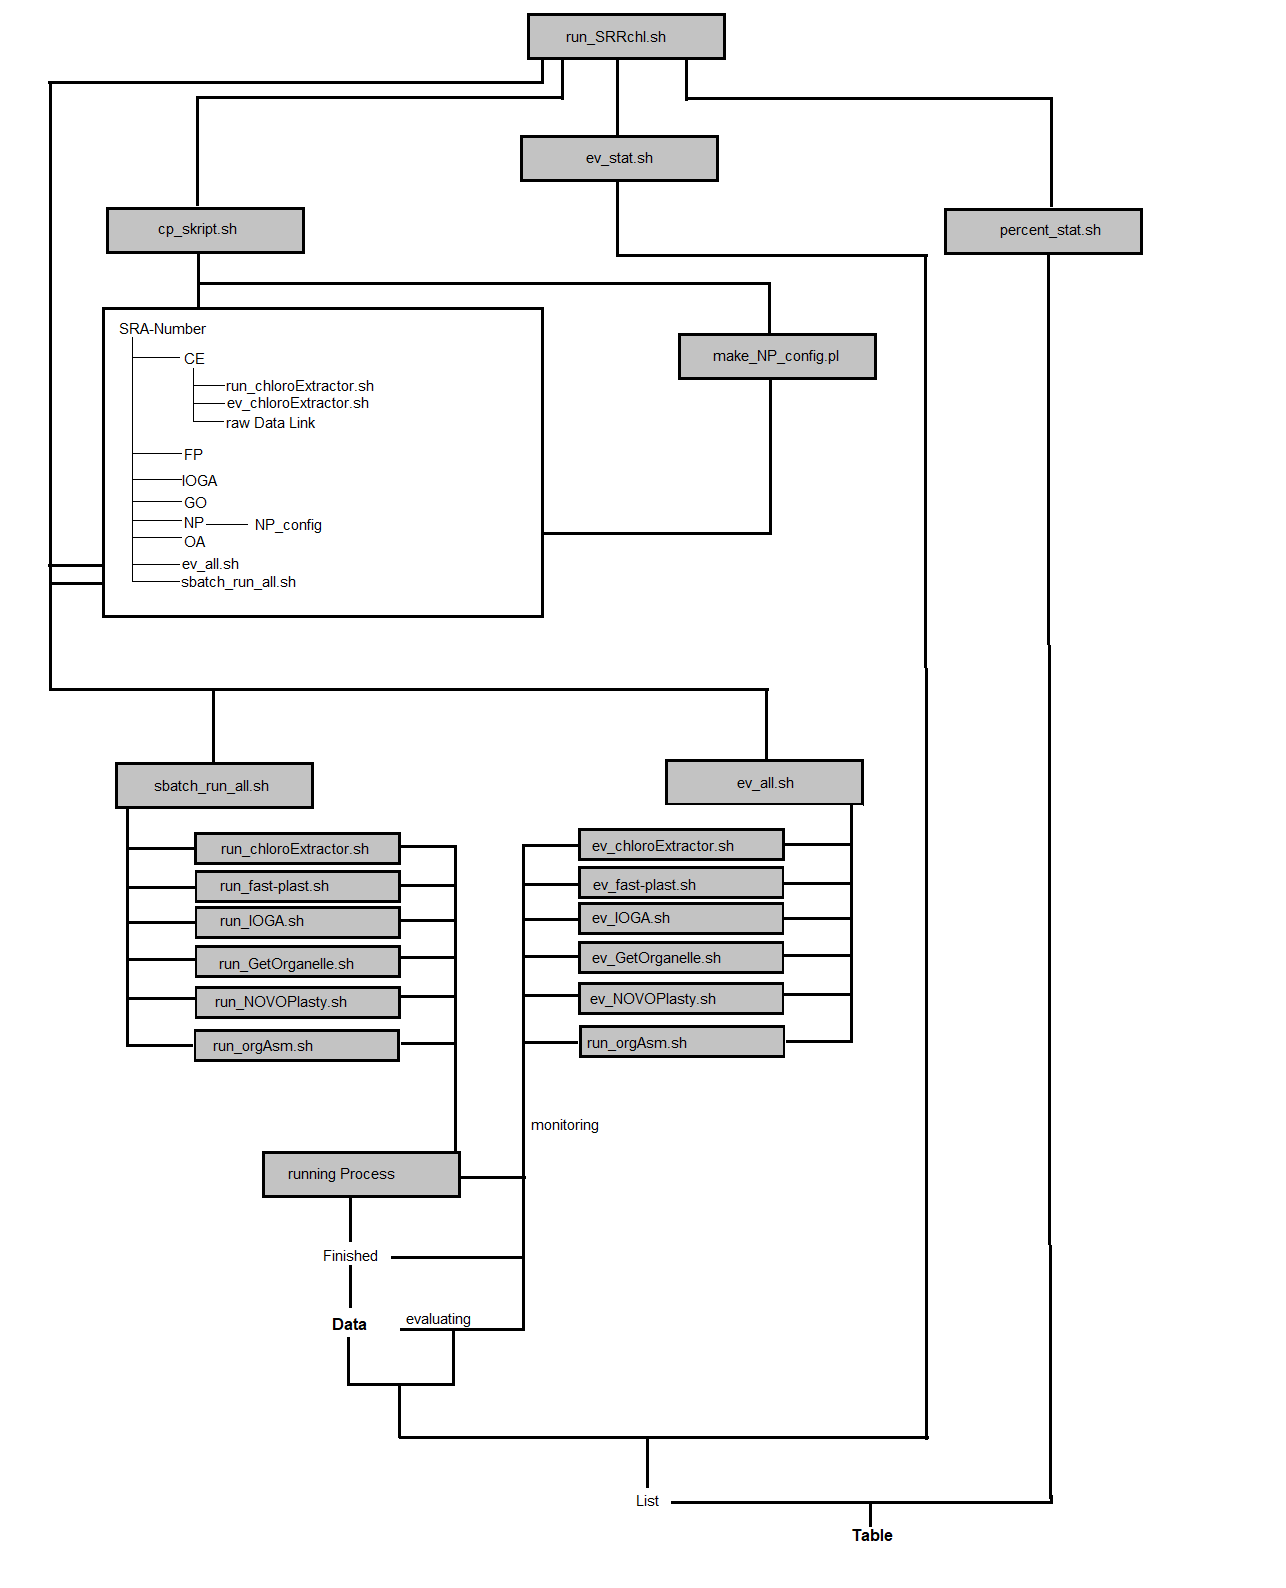
\includegraphics[width=.9\linewidth]{./Diagram_Master.png}
\caption[Automatisierungsskripts]{\textbf{Automatisierungsskripts} Ablauf der verwendeten Skripte um eine Automatisierung zu erwirken, hier wird nur das run\_SRRchl.sh Skript ausgeführt und alle anderen Skripte werden automatisch bis zur Auswertung ausgeführt. So erstellt das cp\_script.sh für jedes Programm einen Unterordner mit den dazugehörigen run und ev Skripts. sbatch\_run\_all.sh startet alle run Skripts und ev\_all.sh startet jedes ev Skript.}
\end{figure}


\subsection{Daten: Simulierte Daten}
\label{sec-4-2}
Die Simulierten Daten, welche mit ART\footnotemark[48]{}\textsuperscript{,}\,\footnotemark[49]{} erzeugt wurden um das verhalten der Programme bei verschiedenen Verhältnissen zu testen, konnten von drei Programmen, dem chloroExtractor, fast-plast und Org.ASM 
bei allen drei Datensätzen geschafft werden. Diese schaffen es einen vollständigen zirkulären Chloroplasten zu bauen. NOVOPlasty baut zwar auch einen kompletten Chloroplasten doch gibt dieser 
nur die drei verschieden Contigs aus (IR, SSC, LSC), und schafft es nicht diese in einen zirkulären Chloroplasten zu vereinen. GetOrganelle wie auch der IOGA schaffen es nicht die
simulierten Datensätze zusammen zu bauen da sie mit einem Fehler abbrechen oder wie im falle des IOGA nach zwei Wochen Laufzeit abgebrochen werden. (s. Tabelle 2) 

\begin{table}[!h]
\caption[Test Datensatz: Simulierte Daten]{\textbf{Test Datensatz: Simulierte Daten} S steht für Success, E für Error, C für Cancelled die angegebene Zahl steht für die Anzahl der Contigs. Bis auf IOGA und GetOrganelle konnten alle anderen Programme die Simulierten Daten zu einem Chloroplasten zusammenbauen, auch wenn im Falle des NOVOPlasty nicht zirkulär. Die IOGA Läufe mit "C" wurden nach zwei Woche Laufzeit abgebrochen.}
\begin{center}
\begin{tabular}{rllllll}
Sim(Genome:Chloroplast) & CE & FP & NP & GO & OA & IOGA\\
 &  &  &  &  &  & \\
\hline
1:10 & S & S & P-3 & E & S & E\\
1:100 & S & S & P-3 & E & S & C\\
1:1000 & S & S & P-3 & E & S & C\\
\end{tabular}
\end{center}
\end{table}

\subsection{Daten: 1001 Genom Projekt, 11 Testdatensätze}
\label{sec-4-3}
Aus den Daten des 1001 Genom Projekts \footnotemark[41]{}\textsuperscript{,}\,\footnotemark[7]{} wurden zunächst elf Testdatensätze verwendet um auch reale Daten auf allen Programmen zu testen.
Von den elf Testdatensätzen des 1001 Genom Projekts konnten sechs verschiedene vollständige zirkuläre Chloroplasten zusammengebaut werden. Von diesen
sechs bringt der fast-plast fünf ein und der chloroExtractor einen. Keines der anderen Programme konnte einen weiteren 
zirkulären Chloroplasten erzeugen (s. Tab.3). Diese elf Datensätze des GetOrganelles wurden per Hand ausgewertet, keiner dieser elf Datensätze konnte einwandfrei mit Bandage
zu einem zirkulären Chloroplasten gebaut werden, da immer kein Ringschluss vorhanden war. (vergleiche Fig.7, Fig. 8)

\begin{figure}
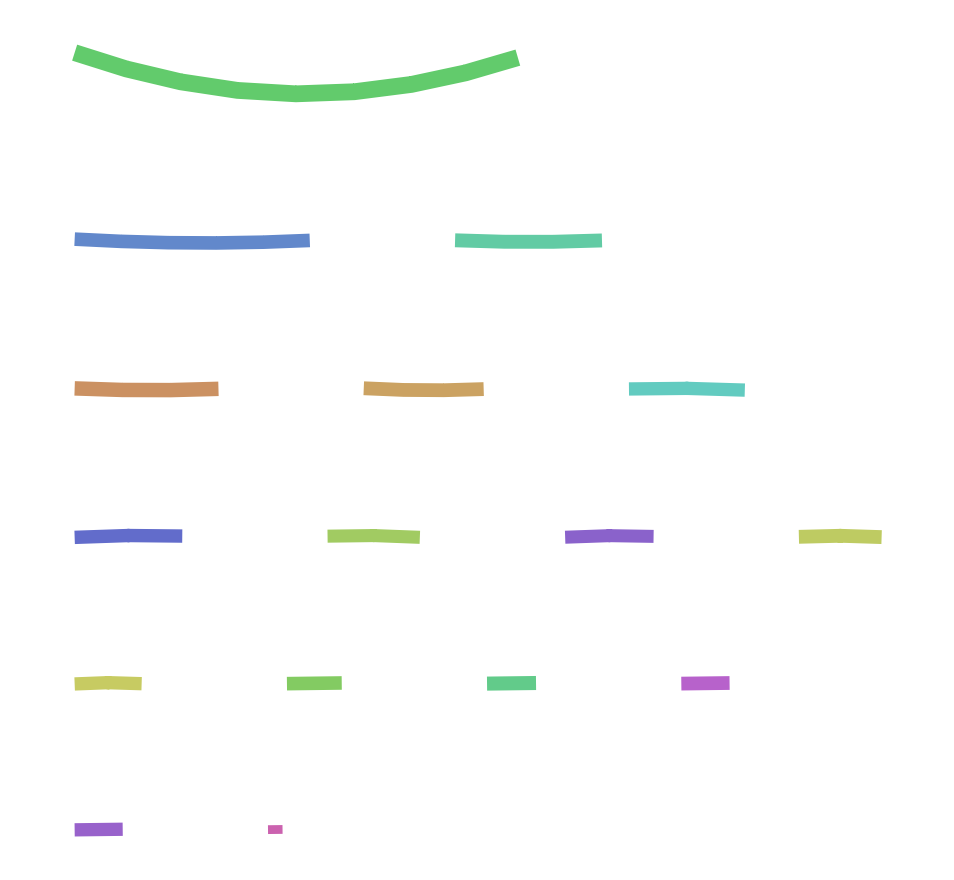
\includegraphics[width=.9\linewidth]{./graph_GO_SRR1945443.png}
\caption[Bandage: GetOrganelle SRR1945443]{\textbf{Bandage: GetOrganelle SRR1945443} Kein Chloroplast erkennbar im fastg Graphen. Keine vernetzung der Contigs per se erkennbar. Dazu im vergleich der graphen des chloroExtractors (Fig. 8)}
\end{figure}
\begin{figure}
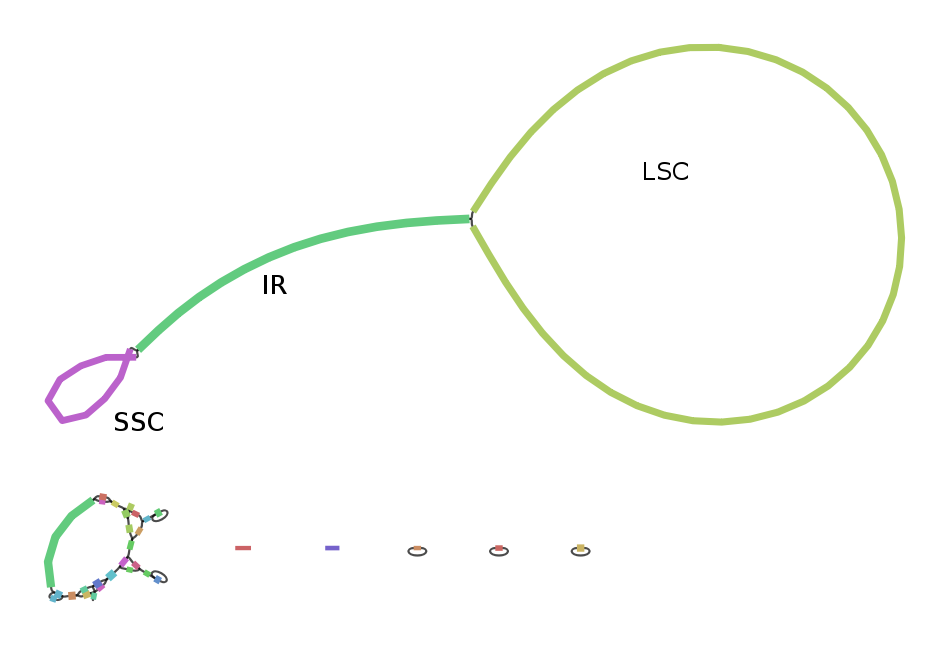
\includegraphics[width=.9\linewidth]{./graph_CE_SRR1945443_1.png}
\caption[Bandage: chloroExtractor SRR1945443]{\textbf{Bandage: chloroExtractor SRR1945443} Chloroplast klar erkennbar, dieser zeichnet sich aus durch einen Großen Kreis (LSC - Gelb), verbunden über eine Linie (IR - Grün) auf einen Kleinen Kreis (SSC - Violett). }
\end{figure}

\begin{table}[!h]
\caption[Test Datensatz: 1001 Genom Project, 11 Datensätze]{\textbf{Test Datensatz: 1001 Genom Project} S steht für Success, E für Error, I für Incomplete, C für Cancelled. Sechs verschiedene Chloroplasten konnten zu einem zirkulären Chloroplasten zusammengebaut werden, dabei werden bereits fünf vom fast-plast abgedeckt und einer wird von chloroExtractor beigesteuert. }


\begin{center}
\begin{tabular}{lllllll}
SRA & CE & FP & NP & GO & OA & IOGA\\
 &  &  &  &  &  & \\
\hline
SRR1945435 & I & I & I & I & E & I\\
SRR1945436 & I & S & I & I & I & I\\
SRR1945437 & I & I & I & I & I & I\\
SRR1945438 & P & S & I & I & E & I\\
SRR1945439 & I & S & I & I & I & I\\
SRR1945440 & I & S & E & I & E & I\\
SRR1945441 & I & S & E & I & I & I\\
SRR1945442 & I & I & I & I & C & C\\
SRR1945443 & S & I & I & I & I & I\\
SRR1945444 & I & I & E & I & I & I\\
SRR1945445 & I & I & E & I & E & I\\
\end{tabular}
\end{center}
\end{table}

\subsection{Daten: GO-Preprint}
\label{sec-4-4}
Um mehr Daten zu testen, wurden alle 57 Datensätze des GetOrganelle Papers \footnotemark[30]{} benutzt. Da der GetOrganelle diese Daten eigentlich erfolgreich schaffen sollte
wurde hier versucht mit dem fcg.pl Skript des chloroExtractors eine Automatisierung der Daten zu erwirken. Doch versucht der GetOrganelle zunächst die die fastg-Graphen
zu verbessern, dies führt dazu dass das fcg.pl Skript nicht mehr funktioniert. So wurden die fastg-Graphen aus SPAdes direkt verwendet, doch ergaben sich hier leider nur
zwei Datensätze als zirkuläre Chloroplasten. Auf Nachfrage beim GetOrganelle Team, hieß es dass, wenn es notwendig war alle Parameter angepasst wurden und dass alle 
Chloroplasten per Hand aus Bandage geholt wurden. 
Von 57 Datensätzen, welche im GetOrganelle Paper verwendet wurden, konnten  insgesamt 40 fertig gestellt werden, diese verteilen sich auf die Programme (s. Tab. 4).
So konnten 35 von 40 Erfolgreichen Datensätzen durch den fast-plast und den chloroExtractor erreicht werden.  Der fast-plast schafft es 31 Chloroplasten Genome komplett
zu bauen, davon sind 17 nur von ihm geschafft worden.( Fig. 9) Der chloroExtractor schafft 14 Chloroplasten, wo von drei nur von ihm geschafft werden. Die zwei Erfolge des GetOrganelles,
mit Hilfe des fcg.pl Skripts des chloroExtractors werden auch nur vom GetOrganelle geschafft. Von den sieben des NOVOPlasty ist einer dabei welcher nur von diesem geschafft wird.
Von den elf des Org.ASM ist auch einer nur von diesem Geschafft worden. Doch wurden einige auch mehrfach geschafft. So sind vier Stück nur von fast-plast und chloroExtractor geschafft worden.
Zwei Stück von fast-plast und Org.ASM, sowie jeweils einer von Org.ASM und NOVOPlasty; chloroExtractor und Org.ASM; fast-plast und NOVOPlasty.
Drei Erfolge teilen sich fast-plast, chloroExtractor und Org.ASM. Sowie jeweils ein Erfolg teilen sich fast-plast, Org.ASM, NOVOPlasty, als auch einer von fast-plast, chloroExtractor und NOVOPlasty.
Zwei Chloroplasten konnten von allen Programmen bis auf GetOrganelle und IOGA gelöst werden (u.a. Fig. 10: SRR5602602 - Laurus nobilis), wobei letzteres Programm nicht einen Erfolg hat(Fig. 9 \& Tab. 4). 
So können bereits 35 von 40 Chloroplasten alleine durch fast-plast und chloroExtractor geschafft werden.

\begin{table}[!h]
\caption[Test Datensatz: GetOrganelle Preprint, 11 Datensätze]{\textbf{Test Datensatz: GetOrganelle Preprint} 40 von 57 Datensätze konnten komplett gelöst werden. 31 Datensätze konnten mit dem fast-plast zu einem Chloroplasten gebaut werden, die 14 die der chloroExtractor schafft enthalten weitere welche nicht vom fast-plast geschafft wurden. Somit konnten mit allen Programmen 74\% gelöst werden, wenn die drei ohne paired Daten herausgerechnet werden und alleine 64\% von diesen 54 von fast-plast und chloroExtractor}
\begin{center}
\begin{tabular}{lrlrrrrl}
Tool & SUCCESS & \% & ERROR & PARTIAL & INCOMPl & NO\_PAIR & Total\\
CE & 14 & \textasciitilde{}26\% & 11 & 17 & 12 & 3 & \\
FP & 31 & \textasciitilde{}57\% & 0 & 18 & 5 & 3 & \\
GO & 2 & \textasciitilde{}4\% & 21 & 26 & 5 & 3 & \\
IOGA & 0 & \textasciitilde{}0\% & 22 & 28 & 4 & 3 & \\
NP & 7 & \textasciitilde{}13\% & 19 & 8 & 20 & 3 & \\
OA & 11 & \textasciitilde{}20\% & 36 & 4 & 3 & 3 & \\
Summary & 40 & \textasciitilde{}74\% & - & - & - & 3 & 57\\
\end{tabular}
\end{center}

\end{table}

\begin{figure}
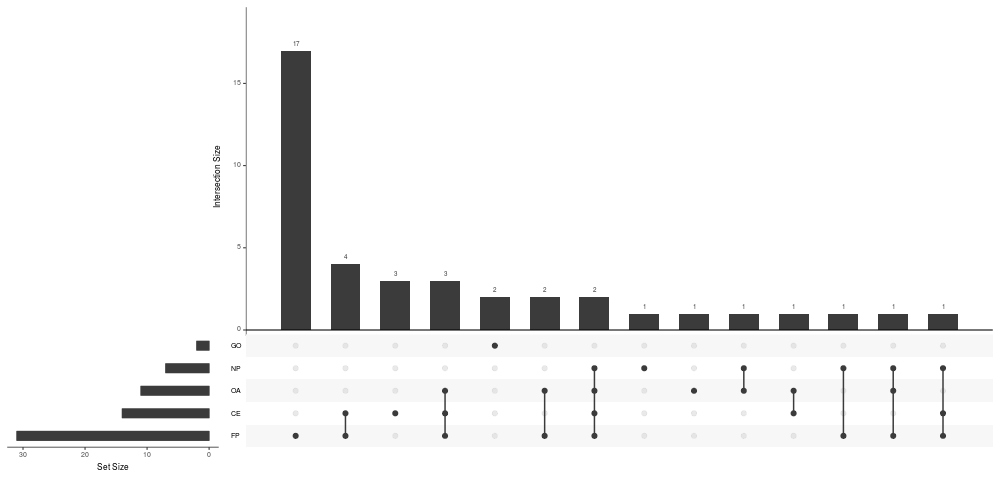
\includegraphics[width=.9\linewidth]{./upset.png}
\caption[Upset Diagramm GO-Preprint]{\textbf{Upset Diagramm GO-Preprint} Hier wird gezeigt wie sich die einzelnen Erfolge auf die 40 Stück aufteilen. So schafft der fast-plast 17 Chloroplasten welches kein anderes Tool schafft. Fast-plast und chloroExtractor haben vier Erfolge gemeinsam, der chloroExtractor schafft drei Chloroplasten welche kein anderes Programm schafft. usw. So werden 35 der geschafften 40 durch fast-plast und chloroExtractor abgedeckt.}
\end{figure}

\begin{figure}
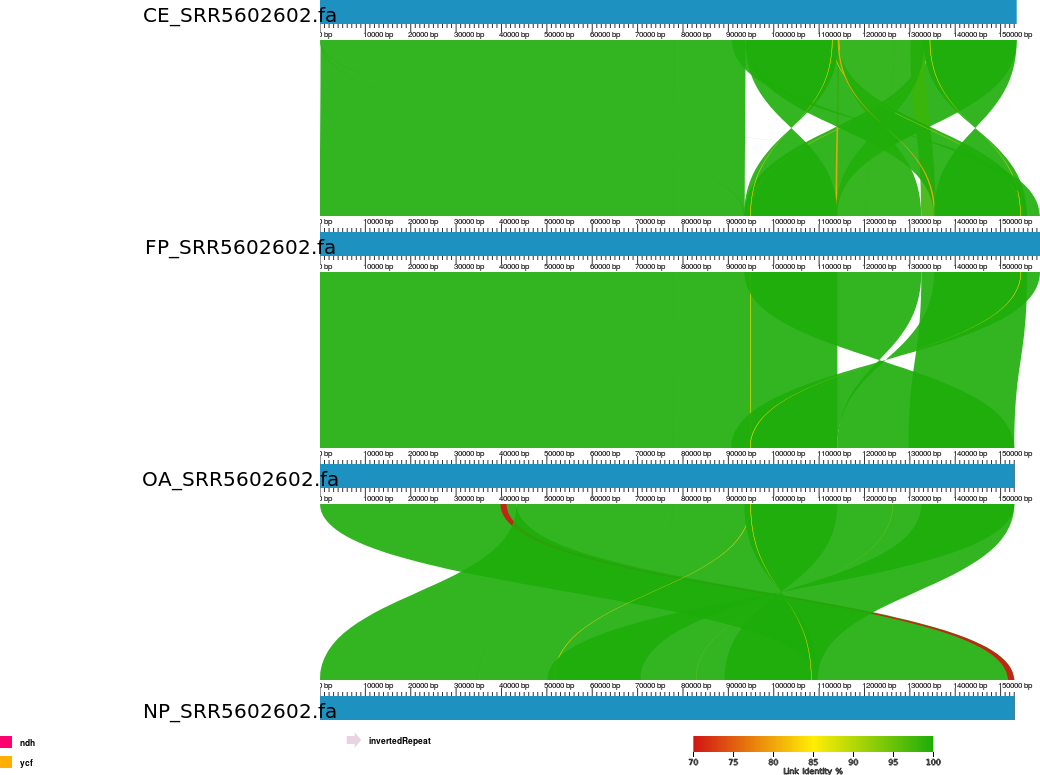
\includegraphics[width=.9\linewidth]{./SRR5602602_1.png}
\caption[AliTV SRR5602602 - Laurus nobilis]{\textbf{AliTV SRR5602602 - \textit{Laurus nobilis}} SRR5602602 -\textit{Laurus nobilis} , SRR5602602 - Laurus nobilis, Daten des GO-Preprints, geschafft von ChloroExtractor, NOVOPlasty, fast-plast und Org.ASM. Orientierung von LSC sowie von SSC und IRs können nicht perfekt aufgelöst werden und können durchaus Verdreht sein.}
\end{figure}

\subsection{Die besten Programme: fast-plast und chloroExtractor}
\label{sec-4-5}
Da aus zeitlichen und hardwaretechnischen Gründen nicht alle Programme weiterverwendet werden konnten, wurde nach Erfolgsrate, Geschwindigkeit und benötigten Ressourcen (s. Tab 5)
gefiltert, am wichtigsten war aber die Automatisierbarkeit der Programme. Bis auf der GetOrganelle konnte für jedes Programm eine Automatisierbarkeit
erwirkt werden ohne Daten außen vor zu lassen. Der GetOrganelle benötigt das öffnen der fastg Datei in einem Visualisierungsprogramm für fastg-Graphen, hier wird Bandage empfohlen.
Bandage hat allerdings eine schlechte Kommandozeilen Anbindung wodurch auch keine Automatisierbarkeit durch Skripts erfolgen konnte.
Es wurde auch versucht mit dem fcg.pl Skript aus dem chloroExtractor, welches genau diesen Schritt im chloroExtractor automatisiert, zu verwenden um auch beim
GetOrganelle eine Automatisierbarkeit zu erreichen. Doch führte dies nur bei sehr wenigen Daten zum Erfolg, da der GetOrganelle die von SPAdes erstellte 
fastg Datei versucht zu verbessern, und die getrimmte Datei nicht mehr vom fcg.pl Skript verwendet werden kann. Dies passiert wohl weil der GetOrganelle beim verbesserten
fastg Graphen versucht Namen und Sequenzen anzupassen, womit das fcg.pl Skript nicht zurecht kommt. Es wurde auch versucht die roh fastg Dateien des GetOrganelle zu benutzen
dies ergab zwar eine Automatisierbarkeit, doch würden so Teile des GetOrganelles, nämlich das verbessern der fastg Datei unterschlagen.
Die Laufzeiten der Programme unterscheiden sich sehr, von 30 Minuten bis über eine Stunde, auch die RAM werte sind sehr unterschiedlich, diese
reichten von wenigen 20 Gigabyte bis zu 60 Gigabyte. All diese Werte sind Durchschnittswerte, da verschiedene Größen von Dateien als Eingabe verwendet wurden. Da nicht alle
Dateien die gleiche Anzahl an Reads hatten, sowie die Größen der einzelnen Reads sich unterschieden. Diese reichten von 75 Basen paare bis zu 300 Basen paare, Anzahl der Reads
und somit Größe der Dateien reichten von eine Millionen Reads bis zu fünf Millionen Reads. Die Laufzeiten sind, vor allem bei Programmen mit vielen Abhängigkeiten, erhört. Da zum nutzen
der Dockercontainer Singularity \footnotemark[53]{} verwendet wurde.    
\begin{table}[!h]
\caption[Laufzeit und Ressourcenverbrauch]{\textbf{Laufzeit und Ressourcenverbrauch} Alle Laufzeiten sind Durchschnittswerte (getrimmtes Mittel), RAM werte zu Peakzeiten. Die Laufzeiten reichen von 30 Minuten (chloroExtractor) bis zu 100 Minuten (IOGA), die RAM Nutzung unterschied sich auch erheblich, diese reichen von 20 GB (chloroExtractor) bis hin zu 60 GB (fast-plast). Aufgrund der Nutzung von verschieden großen Datensätzen können nur Durchschnittswerte Angegeben werden.}
\begin{center}
\begin{tabular}{lll}
Tool & Laufzeit & RAM\\
\hline
CE & \textasciitilde{}  30 min & \textasciitilde{} 20 GB\\
FP & \textasciitilde{}  60 min & \textasciitilde{} 60 GB\\
GO & \textasciitilde{}  40 min & \textasciitilde{} 50 GB\\
IOGA & \textasciitilde{} 100 min & \textasciitilde{} 40 GB\\
NP & \textasciitilde{}  30 min & \textasciitilde{} 30 GB\\
OA & \textasciitilde{}  60 min & \textasciitilde{} 30 GB\\
 &  & \\
\end{tabular}
\end{center}
\end{table}
Die Programme welche in oben genannten Punkte überzeugt haben sind der fast-plast und der chloroExtractor. Der fast-plast benötigt zwar die 
meisten Ressourcen und ist nicht der schnellste, aber hat mit Abstand die größte Erfolgschance. Zudem ist er voll automatisierbar und erreicht 
dies mit den vorgegebenen Standard Parametern. Als zweites Programm wird der chloroExtractor verwendet, dieser ist schnell, Ressourcen arm und hat nach dem
fast-plast die zweit höchste Erfolgsrate. Mit beiden Programmen konnten 35 von den 40 Erfolgen von 57 Chloroplasten der GetOrganelle-Preprint Daten berechnet werden.
Zudem haben diese beiden Programme die wenigsten
Probleme bei der Handhabung wie auch bei der Installation zu beginn gemacht. Sie sind durch die gegebenen Parameter einfach zu verwenden und zu Automatisieren.
Die von den Programmen geschriebenen Log Dateien sind einfach gehalten um dem Ablauf zu folgen und klar verständlich, der fast-plast gibt sogar drei dieser
Dateien aus, da er unterscheidet zwischen Warn- und Fehlermeldungen sowie Standard Meldungen, und eine Datei für den Output der eingebundenen Programme. 
Der chloroExtractor gibt seine Kompletten Meldungen über ein übergeordnetes Programm aus, welche den Ablauf steuert (PipeWrap). Dieses Programm gibt alles auf STDERROR aus und 
kann damit einfach mit geloggt werden. In diesem Fall wurde über die slurm Datei, welche von dem verwendeten queueing System ausgegeben wird, mit geloggt. 
Diese beiden Programme wurden auf allen Daten des 1001 Genom Projekts laufen gelassen, um möglichst viele Chloroplasten zu generieren. 
\subsection{1001 Genom Projekt}
\label{sec-4-6}
Ziel so viele Chloroplasten wie möglich vollautomatisch aus kompletten Genom Datensätze zu erzeugen, wofür zwei Programme ausgewählt worden sind, wurde zunächst auf Datensätzen 
des 1001 Genom Projekt versucht.
Von den 1135 Datensätzen welche im 1001 Genom Projekt gesammelt wurden, konnten 946 Datensätze erfolgreich von NCBI heruntergeladen werden. Die restlichen 189 konnten nicht richtig heruntergeladen werden aufgrund von Downloadfehlern.
Hier handelte es sich um andauerndes Problem, da mehrere male versucht wurde diese Datensätze herunter zu laden. 
Zudem waren 47 Datensätze keine paired end Datensätze, und konnten deshalb nicht verwendet werden. Von diesen 899 restlichen Datensätzen konnten mit dem fast-plast und dem chloroExtractor 303 komplette zirkuläre Chloroplasten 
vollautomatisch gebaut werden, dies entspricht etwa 34\%. (Tab. 6). 
\begin{table}[!h]
\caption[Datensatz: 1001 Genom Project]{\textbf{Datensatz: 1001 Genom Project} SUCCESS, echte zirkuläre Chloroplasten. Error, Fehler oder Abbrüche im Programm. Partial, keine zirkulären Chloroplasten aber Contigs richtig identifiziert. Incomplete, Nicht richtig identifizierte Chloroplasten.}
\begin{center}
\begin{tabular}{lrlrrr}
Tool & SUCCESS & \% & ERROR & PARTIAL & INCOMPLETE\\
CE & 136 & \textasciitilde{}15\% & 54 & 3 & 706\\
FP & 266 & \textasciitilde{}30\% & 29 & 11 & 593\\
Summary & 303 & \textasciitilde{}34\% & - & - & -\\
\end{tabular}
\end{center}
\end{table}

\subsection{Varianz Analyse}
\label{sec-4-7}
Um die Varianz Analyse durchzuführen und vor allem zu überprüfen ob die Assambler bzw. die Programme an sich einen Einfluss darauf haben, indem sie z.B. zufällige Seeds verwenden oder zufällige Daten bevorzugen, wurden 89 Datensätze
des 1001 Genom Projekts verwendet. Diese 89 Datensätze zeichnen sich dadurch aus, dass sowohl der chloroExtractor als auch der fast-plast diese zu vollständigen Chloroplasten zusammengebaut haben. Diese Datensätze
wurden noch zehn weitere Male berechnet. So wurden auf elf mal 89 Datensätzen überprüft welche Einflüsse die Programme auf die Varianz haben. Der chloroExtractor und somit der Assambler SPAdes brachte bei allen elf
Durchläufen die exakt gleichen Sequenzen heraus. Dieses Programm arbeitet also 100\% Reproduzierbar (Fig. 12). Im Gegensatz dazu der fast-plast, dieser schaffte es nicht wieder bei allen elf Durchläufen alle Chloroplasten wieder
korrekt zusammen zubauen, bei bis zu neun verschiedenen Datensätzen konnte kein Erfolgreiches Ergebnis erzielt werden(Fig. 11). Interessanter weiße waren nicht immer die selben Datensätze betroffen, 
so konnten bei einigen Durchläufen
ein Erfolg erreicht werden, bei dem nächsten Durchlauf aber nicht. Ob dies ein Zufalls Effekt des Programms oder der verwendeten Rechner-Infrastruktur ist, konnte nicht überprüft werden.
Die zweite Varianz Analyse bzw. SNP calling wurde auf allen Erfolgreich zusammengebauten Chloroplasten durchgeführt. Das SNP calling ergab dass auf allen 303 Chloroplasten insgesamt 2128 SNPs gefunden wurden. 
Diese Ergebnisse werden für die GWAS Analyse verwendet.
\begin{figure}
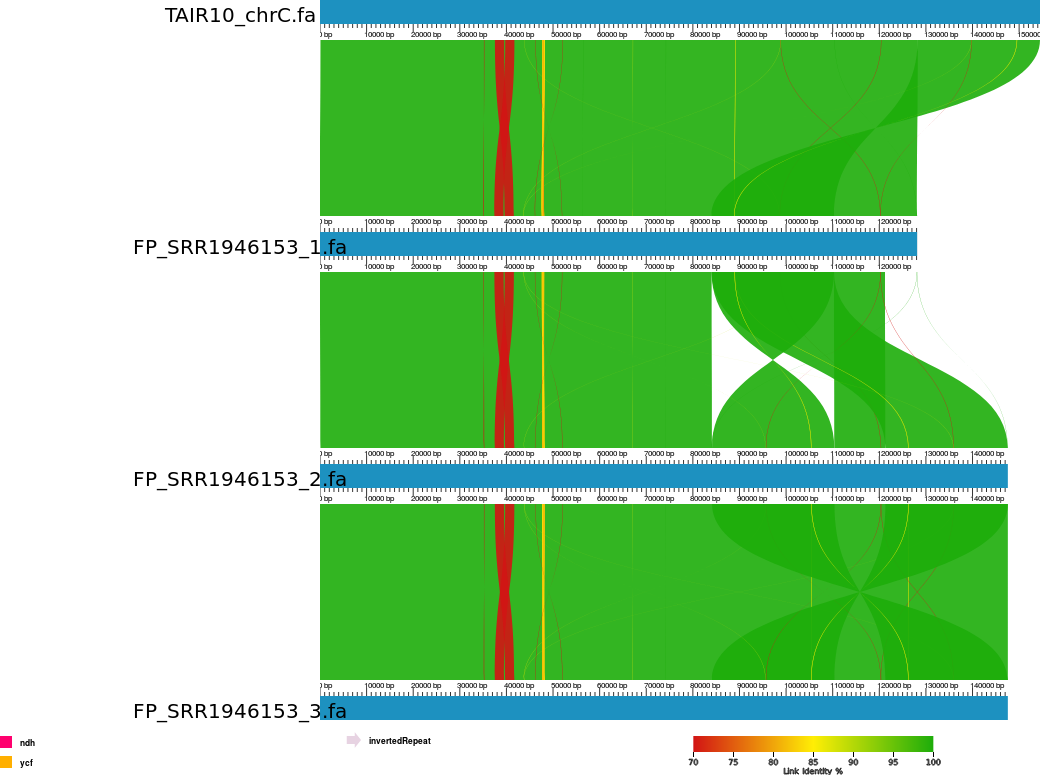
\includegraphics[width=.9\linewidth]{./SRR1946153_FP_1.png}
\caption[fast-plast SRR1946153]{\textbf{fast-plast SRR1946153} Drei verschiedene Läufe auf den selben Daten, der fast-plast schafft einen davon nicht (Lauf 1), den anderen aber schon (2 u. 3). Hier fehlt ein Teil des IR, wodurch auch nicht als Erfolg gewertet wird. }
\end{figure}
\begin{figure}
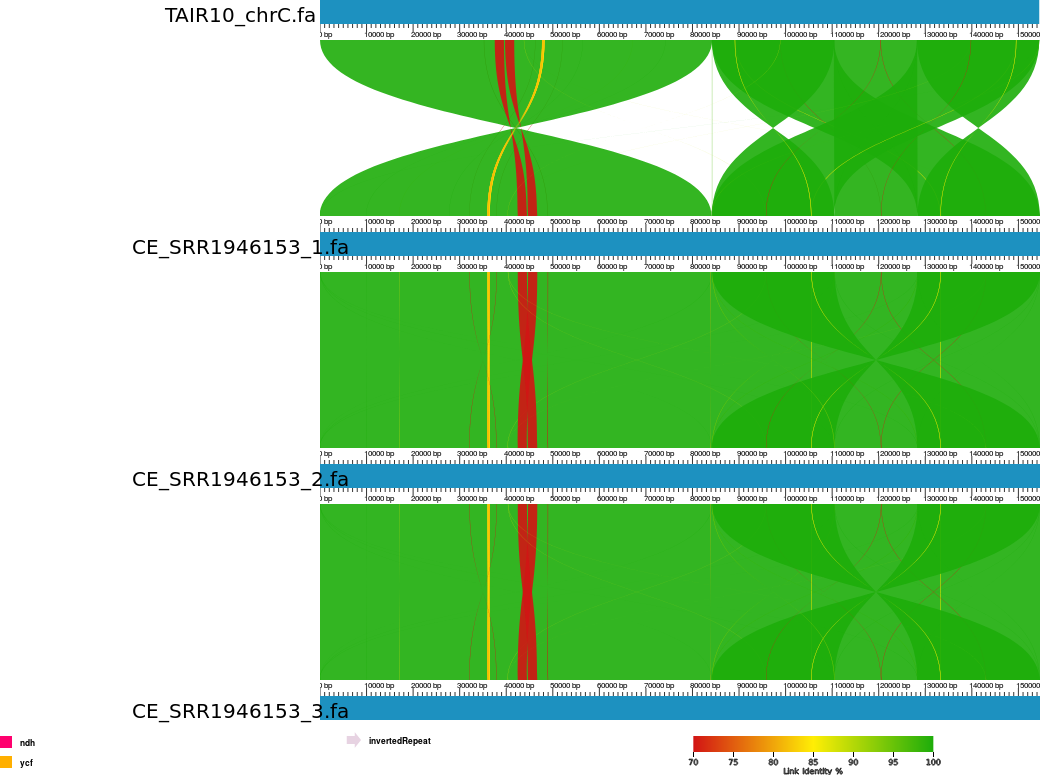
\includegraphics[width=.9\linewidth]{./SRR1946153_CE_1.png}
\caption[chloroExtractor SRR1946153]{\textbf{chloroExtractor SRR1946153} Drei verschiedene Läufe auf den selben Daten, der chloroExtractor bringt das gleiche Ergebnis für alle Durchläufe. Da die Orientierung von LSC, SSC und IR nicht aus short Reads heraus gelesen werden kann, kommt es vor das diese Verdreht sind zur Referenz.}
\end{figure}
\subsection{GWAS}
\label{sec-4-8}
Die GWAS Analyse, welche mit den 303 kompletten Chloroplasten aus den Daten des 1001 Genom Projekts und den 2128 gefunden SNPs durchgeführt wurde, konnte nur auf zwei verschieden Traits berechnet werden. Dies waren 
die Eigenschaften Flowering Time bei 16°C sowie bei 10°C. Dies sind die beiden Traits am besten untersucht sind und deswegen auch die meisten Daten beinhalten. Für alle anderen Traits konnten
keine Berechnungen erstellt werden da die Datenmenge nicht für eine GWAS ausreichend ist. 
\subsection{Struktur Varianz Analyse}
\label{sec-4-9}
Für die Struktur Varianz Analyse konnten keine Ergebnisse erzielt werden, Grund hierfür war unter anderem fehlende Zeit. Aber auch konnten keine Programme gefunden werden welche mit kompletten Chloroplasten
umgehen konnten. Die meisten nutzten direkt Illumina short reads, wie Delly\footnotemark[61]{}\textsuperscript{,}\,\footnote{Rausch T, Zichner T, Schlattl A, et al. (2012) Delly: structural variant discovery by integrated paired-end and split-read analysis. Bioinformatics, \url{https://doi.org/10.1093/bioinformatics/bts378}} oder Breakdancer\footnotemark[62]{}\textsuperscript{,}\,\footnote{Chen K, Wallis JW, McLellan MD, et al. (2009), BreakDancer: an algorithm for high-resolution mapping of genomic structural variation, Nature Methods \url{10.1038/nmeth.1363}}. 

\subsection{Neue Chloroplasten}
\label{sec-4-10}
Aus NCBI wurden 79657 Datensätze heruntergeladen, dies sind alles Pflanzengenome. Diese Liste wurde mit den Einträgen von CpBase ( stand 20.06.2018, 2069 Genome von 942 verschiedenen Spezies )verglichen. Es blieben die Übrig, welche keinen Eintrag in CpBase haben. 
Von diesen 79657 blieben nur 49 Datensätze. Diese wurden auf fast-plast und chloroExtractor benutzt, und es wurden 17 zirkuläre Chloroplasten erfolgreich zusammengebaut (s. Tab. 7). Somit wurden 17 neue Chloroplasten von Spezies
welche zuvor noch keinen genomisch bekannten Chloroplasten hatten erfolgreich erstellt (s. Tab. 8).
\begin{table}[!h]
\caption[Neue Chloroplasten]{\textbf{Neue Chloroplasten} Von den 49 Spezies welche bisher noch keinen Eintrag in CpBase hatte konnten mit Hilfe des fast-plasts und des chloroExtractors 17 neue bisher nicht bekannte Chloroplasten Genome gebaut werden}
\begin{center}
\begin{tabular}{lrrrrl}
Tool & SUCCESS & ERROR & PARTIAL & INCOMPl & Total\\
CE & 4 & 20 & 16 & 9 & \\
FP & 15 & 7 & 22 & 5 & \\
Summary & 17 & - & - & - & 49\\
\end{tabular}
\end{center}
\end{table}

\begin{table}[!h]
\caption[Liste neue Chloroplasten]{\textbf{Liste neue Chloroplasten} Liste von 17 Spezies welche mit Hilfe des fast-plast und des chloroExtractors nun ein bekanntes Chloroplasten Genom besitzen.}
\begin{center}
\begin{tabular}{ll}
SRA & Spezies\\
\hline
DRR057122 & \emph{Momordica charantia}\\
DRR089517 & \emph{Betula chichibuensis}\\
ERR1462646 & \emph{Hippophae rhamnoides}\\
ERR2001942 & \emph{Betula pendula}\\
ERR2003066 & \emph{Potentilla micrantha}\\
ERR2174632 & \emph{Solanum pennellii}\\
ERR2187925 & \emph{Geum urbanum}\\
SRR1503730 & \emph{Agave tequilana}\\
SRR2847417 & \emph{Manihot glaziovii}\\
SRR3194007 & \emph{Artocarpus altilis}\\
SRR3724930 & \emph{Taraxacum S3}\\
SRR4457832 & \emph{Pityopsis pinifolia}\\
SRR5046394 & \emph{Ephedra gerardiana}\\
SRR5464169 & \emph{Trema orientalis}\\
SRR5590327 & \emph{Lagenaria siceraria}\\
SRR5799057 & \emph{Fragaria vesca}\\
SRR5838021 & \emph{Populus deltoides}\\
\end{tabular}
\end{center}
\end{table}

\section{Diskussion}
\label{sec-5}
\subsection{Definition von Success, Einteilung der Erfolge über Genom Länge.}
\label{sec-5-1}
Jegliche Einteilung in die Erfolgs Kategorien: Success, Partial, Incomplete\_high und Incomplete\_low und Error werden von einem Skript übernommen welches zunächst den SeqFilter benutzt um Informationen über diese Datei zu erhalten. 
Der SeqFilter zählt die Sequenzen sowie deren Größe. Das Evaluationsskript des jeweiligen Programms teilt aufgrund dieser Daten in die Kategorien ein (s. Tab. 1). Diese Variante ist zwar voll Automatisiert
doch nicht Fehlerlos, so können Falsch Positive Sequenzen vorkommen. Diese könnte eine Sequenz aus 150 kbp Adenin sein, und das Skript würde es als einen Success ansehen. Die Daten wurden Stichprobenartig überprüft und dies 
kam in diesen Stichproben nicht vor, doch ist es nicht auszuschließen. Um sicher zu gehen müsste jeder erstellter Chloroplast auf eine Referenz gemapt werden oder sogar durch Sequenzierung bestätigt werden. Erste Möglichkeit
wäre nur Rechenaufwand, könnte aber bei Chloroplasten die noch nicht veröffentlicht wurden oder keine Referenz besitzen schwer werden, zweite Möglichkeit ist sehr Kosten intensiv würde aber letzte Zweifel beseitigen. 
Eine Verbesserung des Skripts könnte auch eine strengere Beurteilung sein, zumindest wenn man mehr Grundinformationen hat. So könnten bei den Versuchen mit den \emph{A.thaliana} des 1001 Genom Projekts die Grenzen Strenger gewählt werden, 
da es sich hier immer um die gleiche Spezies handelt. Doch könnten somit die Anzahl der Falsch Negativen erhöht werden, z.B. wenn eine \emph{A.thaliana} Art eine Struktur Variante besitzt mit Verlust eines IR. Die Grenzen wurden 
bewusst großzügiger Gewählt, da dies den größten Teil der Chloroplasten abdecken dürfte. Gerade bei Chloroplasten welche bisher nicht veröffentlicht oder bekannt sind ist eine Abschätzung schwer, da die Größen von Chloroplasten
doch sehr Variieren können. Eine weitere Möglichkeit zu testen ob es sich wirklich um einen Chloroplasten handelt wäre die Verwendung von Benchmarking Universal Single-Copy Orthologs (BUSCO\footnote{Simão FA, Waterhouse RM, Ioannidis P,et al. (2015), BUSCO: assessing genome assembly and annotation completeness with single-copy orthologs.  Bioinformatics, \url{10.1093/bioinformatics/btv351}}), hierzu werden extrem konservierte
orthologe Gene verwendet und überprüft ob diese alle vorhanden sind. Da ein Chloroplast Genom an sich sehr konserviert ist könnte eine Anzahl von Genen genommen werden und diese in einem solchen Modell verwendet werden. 
\subsection{Die Entscheidung für fast-plast und chloroExtractor}
\label{sec-5-2}
Es wurde im Ergebnis Teil erklärt warum gerade der fast-plast und der chloroExtractor weiter verwendet wurden. Doch gibt es auch gründe warum sich speziell gegen andere Programme entschieden wurden. 
So wurde sich gegen den IOGA entschieden, nicht nur weil er langsam ist sondern auch weil er keinerlei Log File während des Prozesses schreibt, erst wenn dieser Komplett beendet ist, so war vor allem zu beginn 
 schwer nachzuvollziehen ob der IOGA nun wirklich noch Arbeitet oder evtl in irgendeinem Loop fest hängt oder sogar aufgehört hat zu arbeiten aber den Prozess nicht beendet. Auch wurde der IOGA zum letzten mal 
vor zwei Jahren geupdated, es scheint also keine Regelmäßige Wartung oder Verbesserung statt zu finden. Es wurde sich auch gegen den NOVOPlasty entschieden, dieser benötigt zwar keine Abhängigkeiten da er komplett 
in Perl geschrieben ist, doch hat dies einige Probleme mit sich gebracht. So werden z.B. nicht alle Read header richtig eingelesen wenn der dazugehörige Reguläre Ausdruck (Regular Expresion - RegEx) nicht komplett passt, dies kam häufiger 
vor da nicht alle Header gleich aufgebaut sind und wohl ein paar nicht abgedeckt wurden. Das zweite Problem mit NOVOPlasty ist die Konfigurationsdatei, diese muss exakt dem Beispiel entsprechen und darf nicht ein Zeichen mehr
oder weniger enthalten, oder gar Zeilen. Da diese Datei nicht über RegEx eingelesen wird sondern Zeile für Zeile durchgegangen wird. So kam es gerade am Anfang vor das der NOVOPlasty gar nicht funktionierte da ein Leerzeichen 
in einer nicht verwendeten Option fehlte. Der NOVOPlasty scheint noch Regelmäßig geupdated zu werden, doch Änderte sich bei diesen Updates der Aufbau der Konfigurationsdatei, weswegen jedes mal das Skript zum erstellen dieser
Datei umgeschrieben werden musste. Auch warf der NOVOPlasty Fehler in denen gesagt wird dass der Seed nicht lesbar oder inkompatibel sei. Doch wurde bei jedem Versuch als Seed die gleiche Datei verwendet, und dieser Fehler trat nur ab und zu auf.
Der Org.ASM brachte zwar erfolgreiche Ergebnisse, im Vergleich würde er auf dem dritten Platz landen, doch gab es einige Probleme bei der Installation. Nur in einem
Dockercontainer mit einigen Tricks konnte es geschafft werden dieses Programm erfolgreich zu installieren. Der GetOrganelle konnte zwar mit dem fcg.pl Skript des chloroExtractors automatisiert werden, doch unterschlägt
dies dann das eigentliche Endprodukt des GetOrganelles, da das verbesserte bzw. getrimmte fastg nicht vom fcg.pl Skript erkannt wurde und deshalb nur das fastg aus SPAdes selbst verwendet werden kann, dies aber häufig schlechter
Ausfällt als das getrimmte oder gar das fastg welches SPAdes im chloroExtractor ausgibt. 
\subsection{Fazit aus der Erfolgschance}
\label{sec-5-3}
Es wurden in dieser Arbeit 303 Chloroplasten Genome von \emph{Arabidopsis thaliana} und 40 von verschiedenen Spezies (GO-Preprint) sowie 17 neue (s. Tab. 8) erstellt. Nimmt man von den Versuchen die gesamt Zahl, so konnten in etwa 30\% der Datensätze zu Chloroplasten Genomen führen.
Dies entspricht Tatsächlich mehr als am Anfang der Arbeit angenommen, hier wurden in etwa 10 - 20\% geschätzt\footnotemark[42]{}. Allerdings auch ohne die anderen Programme, abgesehen von chloroExtractor und org.ASM, getestet zu haben. Nimmt man 
den nur die Erfolgschance von chloroExtractor war diese erste Abschätzung gar nicht so schlecht.   
\subsection{Erhöhen der Erfolgsrate}
\label{sec-5-4}
Es gibt mehrere Möglichkeiten wie eine Erfolgsrate erhöht werden könnte. So könnte versucht werden auf die Daten speziell die Start Parameter festzulegen. Dies würde allerdings einiges an Tests benötigen. 
Auch könnten die Parameter jedes mal 
geändert werden, dann aber unter dem Verlust einer Automatisierbarkeit. In diesen Versuchen wurden verschieden Große Datensätze verwendet, und es lässt sich nicht sagen ob eine Erhöhung dieser einen echten Vorteil bringen würde, 
hierzu müssten alle Daten noch einmal gestartet werden, dann mit erhöhten oder niedrigeren Readmengen. Theoretisch kann dies einen Zuwachs an Erfolg bringen, wenn das verwendete Programm denn auch alle Daten verwendet, 
die es bekommt und nicht
irgendeinen Cutoff ab einer bestimmten Daten bzw. Read Menge hat. Wenn die kompletten Daten verwendet werden würden hätte dies auch den Vorteil das man sicher gehen kann dass die Daten nicht sortiert wurden, indem man diese
einfach nochmal durch mischt. Dies ist wichtig, vor allem bei Programmen welchen einen Cutoff benutzen, denn hier könnte es vorkommen, dass wenn eine Datei sortiert ist Chloroplasten Reads am Ende der Datei liegen und diese somit
gar nicht erst benutzt werden. Dennoch ist zu beachten, je mehr Daten natürlich verwendet werden desto länger brauchen die Programme. Zudem kommt eine erhöhte Download Zeit und evtl. die Zeit die gebraucht wird um die Dateien zu 
mischen bevor diese für die Programme verwendet werden können. 
\subsection{Etablieren einer einfachen scanning Routine}
\label{sec-5-5}
In dieser Arbeit wurde gezeigt das eine voll Automatische Lösung für das scannen von Chloroplasten in Pflanzen Genom Daten möglich und auch erfolgreich ist. Die hier verwendeten Skripte können frei verwendet und angepasst werden. 
Doch kann dies alles auch in einem kompletten Dockercontainer benutzt werden. Der chloroExtractorTeam Screening Container\footnote{\url{https://github.com/chloroExtractorTeam/screening_container}}, kann verwendet werden um komplett automatisch die Daten von NCBI herunter zu laden, diese zu mischen
(mit einem festen Seed) und dann den chloroExtractor und den fast-plast zu verwenden um diese Daten zu verarbeiten. Hierzu muss lediglich der Container gestartet werden und der run.sh Befehl mit der Passenden SRA Nummer gegeben 
werden. Dieser Container wird gerade verwendet um weitere 12393 Datensätze zu durchsuchen und Chloroplasten zu bauen. Diese Container ist sehr einfach zu benutzen, und alles was dafür gebraucht wird ist Docker\footnotemark[44]{} oder ein Programm
welches Dockercontainer ausführen kann wie z.B. Singularity\footnotemark[53]{}. 
\subsection{GWAS}
\label{sec-5-6}
Es wurde eine GWAS Studie auf den 303 \emph{A.thaliana} Chloroplasten durchgeführt, doch konnte dies nur auf zwei verschiedenen Eigenschaften berechnet werden. Hierzu gehört die Flowering Time bei 16°C sowie bei 10°C. 
Die restlichen Arapheno Traits konnten nicht berechnet werden. Dies ist vor allem der Fall da zu wenige Daten zur Verfügung stehen, sowohl von unserer Seite aus als auch von der Eigenschaften Seite aus. Eigenschaften wie
Größen, Blütenbreite oder Form sind nicht gut genug Katalogisiert um eine geringe Datenmenge, wie sie hier benutzt wurde abzudecken. Dies heißt nicht das keinerlei Assoziation zwischen Chloroplasten Varianz und diesen Eigenschaften besteht.
Dies zeigt lediglich dass noch mehr Daten benötigen werden um diese GWAS Studie zu beenden‌.
\subsection{Struktur Varianz}
\label{sec-5-7}
Es wurde angenommen, dass ein kompletter Chloroplast für eine Struktur Varianz Analyse einen großen Vorteil bringt im Vergleich zu Illumina short Reads. Diese sind häufig zu kurz um große Invertierungen oder neu Anordnungen zu 
überspannen. Leider konnte diese Annahme nicht überprüft werden, da zu wenig Zeit vorhanden war. Als auch Programme, welche eine solche Analyse durchführen nicht erfolgreich benutzt werden konnten 
\subsection{Fazit und Zukunftsaussichten}
\label{sec-5-8}
Chloroplasten Genome können vielseitig verwendet werden und mit der immer steigenden Anzahl dieser Genome können mehr und mehr Analysen durchgeführt werden. Hier wurde eine Möglichkeit gezeigt wie man solche Chloroplasten Genome
aus bereits existierenden Daten bauen kann. Dies ist aber nur möglich da alle Daten danke Open Science verfügbar waren. Es wurden 360 Chloroplasten aus bereits vorhandenen Daten erzeugt, die meisten aus \emph{Arabidopsis thaliana}
Daten, die vom 1001 Genom Projekt verwendet wurden. Es wurden aber auch 17 Neue Chloroplasten Genome erzeugt. Zudem wurde ein erster Ausblick auf die verschiedenen Analysen gegeben welche mit Chloroplasten Genomen möglich sind.
Schaut man sich die Updates der verschiedenen Programme an, so wird ein Teil davon immer noch geupdated bzw. verbessert. Je mehr Chloroplasten Genome mit der Zeit verfügbar werden, desto 
mehr Analysen können mit diesen Chloroplasten durchgeführt werden. So zeigte sich hier bei dem versuch einer GWAS, dass es bei zu wenigen Daten zu Problemen kommen kann. 
Diese Arbeit zeigt vor allem eines, es ist durch Automatisierung möglich Chloroplasten Genome aus Pflanzlichen Sequenzdaten zu bauen. Dank der Automatisierung ist hier lediglich Rechenpower von Nöten. So können in Zukunft
noch viel mehr Chloroplasten Genome erzeugt werden.
\section{Abbildungs- und Tabellenverzeichnis}
\label{sec-6}
\listoffigures

\listoftables
\clearpage
\section{Anhang}
\label{sec-7}
\subsection{Dockercontainer}
\label{sec-7-1}
\begin{table}[!ht]
\caption[Dockercontainer]{\textbf{Dockercontainer} Alle erstellten Dockercontainer stehen zur freien Verfügung.}
\begin{center}
\begin{tabular}{ll}
Programm & Dockerhub link\\
\hline
chloroExtractor & \url{https://hub.docker.com/r/chloroextractorteam/chloroextractor/}\\
 & Build: b5uvjvdnbcyndhjngua85nv\\
fast-plast & \url{https://hub.docker.com/r/chloroextractorteam/fast-plast_docker/}\\
 & Build: bgrmngfwpil4sk2kezi9f\\
NOVOPlasty & \url{https://hub.docker.com/r/chloroextractorteam/novoplasty_docker/}\\
 & Build: bf9adepndze96bcnteyeabk\\
IOGA & \url{https://hub.docker.com/r/chloroextractorteam/ioga_docker/}\\
 & Build: bwnf4xtzhohfcstqjqsvqvw\\
GetOrganelle & \url{https://hub.docker.com/r/chloroextractorteam/getorganelle_docker/}\\
 & Build: bwt3bus2r7utsjpgrmjmjuc\\
Org.ASM & \url{https://hub.docker.com/r/chloroextractorteam/org.asm_docker/}\\
 & Build: bmcx88c2d79orvuykgivy4q\\
 & \\
Screening Container & \url{https://hub.docker.com/r/chloroextractorteam/screening_container/}\\
 & Build: bdsankaqpukcgfmkmdq9yud\\
\end{tabular}
\end{center}
\end{table}
\begin{table}[!ht]
\caption[Git Links]{\textbf{Git Links} Alle verwendeten Programme stehen zur freien Verfügung.}
\begin{center}
\begin{tabular}{ll}
Programm & git link\\
\hline
chloroExtractor & \url{https://github.com/chloroExtractorTeam/chloroExtractor}\\
 & \\
fast-plast & \url{https://github.com/mrmckain/Fast-Plast}\\
 & \\
NOVOPlasty & \url{https://github.com/ndierckx/NOVOPlasty}\\
 & \\
IOGA & \url{https://github.com/holmrenser/IOGA}\\
 & \\
GetOrganelle & \url{https://github.com/Kinggerm/GetOrganelle}\\
 & \\
Org.ASM & \url{https://git.metabarcoding.org/org-asm/org-asm}\\
 & \\
 & \\
Screening Container & \url{https://github.com/chloroExtractorTeam/screening_container}\\
 & \\
\end{tabular}
\end{center}
\end{table}


\clearpage
\subsection{Danksagung}
\label{sec-7-2}
Ich möchte allen Danken, welche mich in meiner Zeit als Student vor allem in den letzten Semestern unterstützt haben.
Zunächst Danke ich dem kompletten CCTB, in dem ich in den letzten Semestern mit mehr als nur Kollegen zusammenarbeiten durfte.
Hier möchte ich im besonderen meinen Betreuern Markus Ankenbrand und Jörg Schulz danken, welche sich die Zeit nehmen müssen diese 
Arbeit zu korrigieren und immer mit Rat zur Seite standen. Speziell möchte ich auch meinen ganz besonderen Dank an Frank Förster aussprechen, der uns mehr als nur beratend zur Seite stand und mehrere Nächste 
geopfert hat um unseren chloroExtractor zu verbessern und zu fixen. 
Auch möchte ich aber meiner kompletten Familie danken, meinen Eltern Roland und Maria, sowie meinen beiden Brüdern Florian und Christopher, sowie meinem Bruder im Geiste Martin "Löwe" Piekar, sowie natürlich den Damen
welche es mit diesen drei Chaoten aushalten, die da wären Vanja, Julia und Charlotte. Natürlich danke ich auch all meinen anderen Freunden welche es mit mir all die Jahre ausgehalten haben, und dies planen noch weiter zu tun,
so wie der World of Warcraft Community, der Gilde Maestri delle Arte und dem Raid Invictus, welche mich immer gut unterhalten haben, und das ein oder andere mal evtl. auch zu viel von der Arbeit abgehalten haben.
Auch geht mein Dank an Kaffee, vielen dank für Substitution von Schlaf mit Koffein. 


\subsection{Skripte}
\label{sec-7-3}
Alle verwendeten Skripte können gefunden werden unter:
\\
\url{https://github.com/chloroExtractorTeam/chloroplast_landscape/tree/Documentation_SPfaff}
Zudem sind diese auf der beiliegenden CD zu finde.
\subsection{Tabellen}
\label{sec-7-4}
Alle Ergebnis Tabellen können eingesehen werden unter: 
\\
\url{https://github.com/chloroExtractorTeam/chloroplast_landscape/tree/Documentation_SPfaff}
Zudem sind diese auf der beiliegenden CD zu finde.
\clearpage
\section*{Eigenständigkeitserklärung}
ERKLÄRUNG gemäß ASPO vom 5.8.2009 § 23 Abs. 10\\[10mm]
Hiermit versichere ich, dass ich vorliegende Arbeit selbstständig verfasst, keine anderen als
die angegebenen Quellen und Hilfsmittel benutzt und die Arbeit bisher oder gleichzeitig
keiner anderen Prüfungsbehörde unter Erlangung eines akademischen Grades
vorgelegt habe.\\[20mm]
Würzburg, \today \hfill Simon Pfaff
\clearpage
% Emacs 24.5.1 (Org mode 8.2.6)
\end{document}
